\documentclass[11pt]{article}

% "review" hides authors; use "final" for the submitted version.
\usepackage[final]{acl}

\usepackage{times}
\usepackage{latexsym}
\usepackage[T1]{fontenc}
\usepackage[utf8]{inputenc}
\IfFileExists{microtype.sty}{\usepackage{microtype}}{}
\IfFileExists{inconsolata.sty}{\usepackage{inconsolata}}{}
\usepackage{graphicx}
\usepackage{booktabs}
\usepackage{amsmath,amssymb}
\usepackage{tikz}
\usetikzlibrary{positioning,arrows.meta,decorations.pathreplacing,fit}
\graphicspath{{figs/}}

\title{SIH Behind the Stage: A Causal Audit of Semantic Induction Heads}

\author{Maxim Golubkov \\
  Tel Aviv University \\
  \texttt{TODO@mail.tau.ac.il} \\\And
  Daniella Simonovsky \\
  Tel Aviv University \\
  \texttt{TODO@mail.tau.ac.il} \\}

\begin{document}
\maketitle

\begin{abstract}
TODO (written last).
\end{abstract}

\section{Introduction}
\label{sec:intro}
TODO (written last).

\section{Background and Related Work}
\label{sec:background}

Two lines of work assign functions to attention heads. The first \emph{describes} a
head by its attention pattern and weights. The second \emph{intervenes} on the head
and measures what changes in the output. Semantic induction heads were defined in the
first way; we audit them with the tools of the second.

\subsection{Induction heads and semantic induction heads}
\label{sec:sih}

\paragraph{Induction heads.}
An attention head can be split into a QK circuit, which chooses where the head
attends, and an OV circuit, which determines what it writes
\citep{elhage2021mathematical}. An \emph{induction head} uses the QK circuit to attend
from a repeated token $[A]$ to the token $[B]$ that followed its earlier occurrence,
and the OV circuit to raise the logit of $[B]$. The behaviour is defined on controlled
repeated sequences, and its importance for in-context learning was established by
ablation \citep{olsson2022induction}. Appendix~\ref{app:ih} gives the fuller picture,
including retrieval heads \citep{wu2024retrieval}.

\paragraph{Semantic induction heads.}
\citet{ren2024semantic} keep the same QK/OV template but let the written token differ
from the attended one. Given a relation triplet $(t_s, r, t_o)$ in the context---a
\emph{head} token $t_s$, a relation $r$ and a \emph{tail} token $t_o$---a
\emph{semantic induction head} (SIH) is a head that, at a later current token $t_j$,
attends to $t_s$ and raises the logit of $t_o$ (Figure~\ref{fig:ri}). The
\emph{relation index} (RI) turns this into a score. Let $p^{h,j}=\mathrm{softmax}(x_j
W^h_{OV} W_U)$ be the vocabulary distribution obtained by pushing the current token's
input embedding $x_j$ through head $h$'s OV weights and the unembedding, restricted to
the tokens seen so far and centred at zero. Then
\begin{equation}
\label{eq:ri}
\mathrm{RI}_h \;=\; \operatorname*{mean}_{(T,j)\,:\,\text{$h$ attends to } t_s}
\;\frac{q^{h,j}_{t_o}}{\sum_{k\le j} q^{h,j}_{t_k}},
\end{equation}
where $q^{h,j}_t=\max(0,\,p^{h,j}_t-\bar p^{h,j})$ and the mean runs over all
(triplet, position) pairs at which the head's attention argmax is $t_s$ by a fixed
margin. The index is the share of the head's positive output mass that lands on the
tail token; heads with a high index for a relation are called SIHs. The authors also
report that in a model they train, the index of some heads rises at the training
stage where few-shot pattern discovery emerges, and conclude that SIHs play a crucial
role in in-context learning. Appendix~\ref{app:ri} restates the definition exactly.

\begin{figure}[t]
\centering
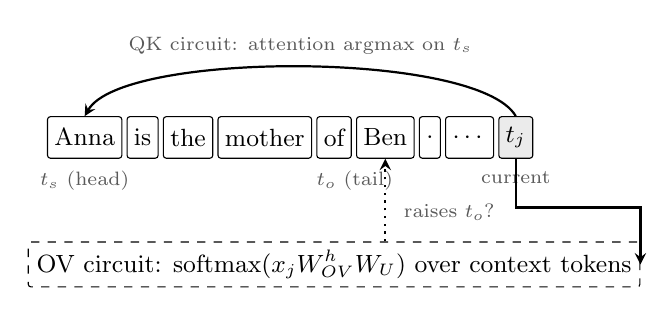
\begin{tikzpicture}[
  tok/.style={draw, rounded corners=1pt, minimum height=1.5em, inner sep=2.5pt, font=\small},
  lab/.style={font=\scriptsize, text=black!65},
  >=stealth, node distance=1.5pt]
\node[tok] (t1) {Anna};
\node[tok, right=of t1] (t2) {is};
\node[tok, right=of t2] (t3) {the};
\node[tok, right=of t3] (t4) {mother};
\node[tok, right=of t4] (t5) {of};
\node[tok, right=of t5] (t6) {Ben};
\node[tok, right=of t6] (t7) {.};
\node[tok, right=of t7] (t8) {$\cdots$};
\node[tok, right=of t8, fill=black!8] (t9) {$t_j$};
\node[lab, below=1pt of t1] {$t_s$ (head)};
\node[lab, below=1pt of t6, xshift=-11pt] {$t_o$ (tail)};
\node[lab, below=1pt of t9] {current};
% QK: arc above the tokens
\draw[->, thick] (t9.north) to[out=120, in=60, looseness=0.45]
  node[lab, above, pos=.5, yshift=1pt] {QK circuit: attention argmax on $t_s$} (t1.north);
% OV: down from t_j, project, raise the tail token
\node[tok, dashed, below=1.05cm of t5, inner sep=3pt] (voc)
  {OV circuit: $\mathrm{softmax}(x_j W^h_{OV} W_U)$ over context tokens};
\draw[->, thick] (t9.south) -- ++(0,-0.62) -| (voc.east);
\draw[->, thick, dotted] (voc.north -| t6) -- node[lab, right=3pt, pos=.35] {raises $t_o$?} (t6.south |- t6.south) ;
\end{tikzpicture}
\caption{The relation index. For a relation (Anna, mother-of, Ben) stated in the
context, a head scores on a later current token $t_j$ if its attention argmax falls
on the head token $t_s$ and the vocabulary projection of its OV output, computed from
the \emph{input embedding} of $t_j$, puts a large share of its mass on the tail token
$t_o$. The projection is read at $t_j$, not at the attended position.}
\label{fig:ri}
\end{figure}

\paragraph{What the original study does not establish.}
The SIH evidence is descriptive. \emph{(i)} No head is intervened on, so it is not
tested whether high-RI heads are needed for the model to use a relation, or whether
the heads that are needed have a high RI. \emph{(ii)} The training-dynamics claim
rests on co-timing between a selected set of rising indices and a behavioural
transition, in a separately trained model; it is not shown that the heads whose
index rises are the heads that carry the ability, nor that they are the final SIHs.
\emph{(iii)} The index projects the \emph{raw embedding} of the current token, an
approximation borrowed from attention-only models. In a deep model the head's value
input is a contextual residual, and what the head writes at $t_j$ depends on the
positions it attends to, not on the embedding at $t_j$. There is no evident reason
for such a score to track the head's contribution. \emph{(iv)} The index has no
control (the tail competes only with all earlier tokens) and no null distribution, so
``high'' has no reference. Appendix~\ref{app:ri} details each point against the
original text. We address (i) by causal measurement of every head
(\S\ref{sec:method-causal}); (iii) and (iv) by re-implementing the RI with matched
controls and a null calibration (\S\ref{sec:method-ri}) and by testing whether the
head's actual contextual input repairs the score (\S\ref{sec:results-char}). We do not
study training dynamics; (ii) remains a limitation of the original evidence.

\subsection{Causal interventions on heads}
\label{sec:rw-patching}

\emph{Activation patching} replaces the activation of one component on a clean input
with its activation on a minimally different corrupted input and measures the change
in the model's output \citep{wang2023ioi,heimersheim2024patching}. Run in the
\emph{noising} direction (corrupted activation into the clean run) it measures how
much of the output depends on the component; run in the \emph{denoising} direction
(clean activation into the corrupted run) it measures how much the component alone
restores. \citet{heimersheim2024patching} note that the two are not symmetric and
recommend reporting both. The choice of metric matters as much as the intervention:
\citet{zhang2024bestpractices} show that logit difference between the correct and the
corrupted answer is more informative and less brittle than probability or accuracy,
and that conclusions about which components matter can flip between metrics. The
indirect-object-identification (IOI) study of \citet{wang2023ioi} established the
per-head, per-position form of these tools on GPT-2 small and introduced the
vocabulary that later work inherited: \emph{name movers} that copy the answer,
\emph{negative name movers} that suppress it, and \emph{backup} heads that activate
only when others are removed. We use noising and denoising head patching with the
logit-difference metric throughout (\S\ref{sec:setting}), at all prompt positions and
at the answer position separately, and we split a head's patched output into the
attention pattern and the values it reads, as in the QK/OV decomposition of
\S\ref{sec:sih}.

\subsection{Reading what a head writes}
\label{sec:rw-readout}

Intervention tells us that a head matters; a second family of tools asks what it
contributes. \emph{Direct logit attribution} projects a head's output vector onto the
unembedding to see which tokens it promotes \citep{elhage2021mathematical,wang2023ioi};
the relation index of \S\ref{sec:sih} is a weight-only version of this projection that
uses the current token's embedding instead of the head's actual output. Behavioural
\emph{fingerprints} test a head on controlled synthetic inputs: prefix-matching and
copying scores on repeated random sequences \citep{olsson2022induction} and
needle-retrieval scores on key--value contexts \citep{wu2024retrieval} identify
induction and retrieval heads independently of any natural-language task. Finally,
\emph{Patchscopes} \citep{ghandeharioun2024patchscopes} decode a hidden
representation by injecting it into a separate prompt whose continuation exposes its
content; the method reads representations, not head contributions, so head
attribution requires comparing intact and head-intervened representations under the
same readout. We use all three: the contextual output projection and its
raw-embedding counterpart side by side, both synthetic fingerprints on every head in
our inventory, and a controlled Patchscopes-style readout of the sites where our
strongest head writes.

\subsection{From heads to circuits}
\label{sec:rw-circuits}

A list of important heads is not a mechanism. \emph{Path patching}
\citep{wang2023ioi} isolates a single edge: the output of a source component is
patched only along its path into a chosen receiver (for a head, its query, key or
value input), so an effect on the output shows that the receiver uses what the source
wrote. \citet{conmy2023acdc} automate this search, pruning edges whose removal does
not change a task metric, and \citet{haklay2025position} show that edges must be
indexed by token position: the same head can be essential at one position and inert
at another, and position-agnostic circuits miss this. How a discovered circuit is
judged also matters. \citet{hanna2024faithfulness} argue that overlap with a
hand-found reference is the wrong target and that a circuit should be evaluated by
\emph{faithfulness}: how much of the full model's behaviour it reproduces when
everything outside it is ablated, checked with several ablation schemes and metrics.
Our Stage-4 design follows these three points: edges are tested by path patching
into keys and values at the source's fact positions, routes are indexed by position,
and the resulting head mechanism is evaluated by faithfulness on families held out
from every earlier stage.

\subsection{The gap}
\label{sec:rw-gap}

The two lines of work reviewed above rarely meet on the same heads. Descriptive
criteria propose what a head does from its weights or attention; circuit studies
find what heads do by intervening on a task. For semantic induction heads the two
have not been connected: \citet{ren2024semantic} show that some heads stand out on
their relation index and read this as evidence that the heads ``encode'' relations,
but the index is not checked against the model's behaviour. This work examines the
relation between the descriptive SIH criterion and the causal mechanisms that
support the use of in-context relations. Using head-, group- and path-level
interventions in OLMo-2-7B, we characterize the overlap and the gaps between
identification by RI and contribution to behaviour on a relational task; a
complementary analysis across training checkpoints separates the development of
attention routing from the development of the conditional relation index.

\section{Experimental Setting}
\label{sec:setting}

\paragraph{Model.}
All experiments use the base OLMo-2-1124-7B \citep{olmo2024olmo2} (32 layers, 32
heads per layer, $d_{\text{model}}{=}4096$), revision
\texttt{7df9a82}, without fine-tuning, in fp16. We chose OLMo-2 because its training
checkpoints are public, which the developmental analysis needs, and because at 7B it
is the largest model on which our per-head, per-position interventions were
affordable on the available GPUs (Appendix~\ref{app:compute}).

\paragraph{Task.}
The model must retrieve a relation stated in its context. A prompt contains four
in-context demonstrations followed by a test block of four facts of the form
``$\langle$mother$\rangle$ is the mother of $\langle$child$\rangle$.'' and the
question ``Question: Who is the mother of $\langle$child$\rangle$? Answer:''. The
answer is the mother named in the \emph{query fact}, the fact whose child is asked
about. All names are invented, so the answer cannot come from parametric knowledge,
and the test block always contains a second, structurally identical fact whose mother
is the \emph{distractor}. This is the SIH setting of \S\ref{sec:sih}---a head token
(the child), a relation (mother-of) and a tail token (the mother)---with the relation
annotated at construction time rather than by a parser.

\paragraph{Data.}
We generated 200 \emph{families} of invented names. Each family yields a
\emph{clean} prompt, a \emph{corrupted} twin in which the two answer-side mothers are
swapped inside the fact lines (so the distractor becomes the answer while every token
position and mention count is unchanged, as activation patching requires), and a
\emph{reorder} variant with shuffled fact lines; each in two fact orders.
Appendix~\ref{app:data} shows a complete example. Before any intervention we
verified that the model performs the task: 4-shot accuracy on clean, corrupted and
reordered prompts, in both orders, is 93\%, 94\% and 89\% of families. The 176
families correct on clean and corrupted prompts in both orders are split by family
id: 89 \emph{discovery} families (178 clean/corrupted pairs) for all scoring and
selection, and 87 \emph{held-out} families reserved for the final faithfulness and
generalization tests. A fixed subset of 20 discovery families (40 pairs) is used
where a measurement must cover all 1,024 heads.

\paragraph{Metric and intervention scopes.}
Following \citet{zhang2024bestpractices}, the outcome of every intervention is the
logit difference between the clean answer $y_c$ and the corrupted answer $y_r$,
\begin{equation}
\label{eq:metric}
M(x)=\operatorname{logit}(y_c\mid x)-\operatorname{logit}(y_r\mid x),
\end{equation}
evaluated at the first token at which the two answers differ (a shared prefix, when
one exists, is teacher-forced). The sign is fixed to the clean answer on both inputs,
so $M(x_c)>0$ and $M(x_r)<0$ mean that the model follows the stated fact. The
\emph{importance} of head $h$ is the drop in $M$ on the clean prompt when the head's
output is replaced by its output on the corrupted twin, $I_h=M(x_c)-M(x_c;a_h
\leftarrow a^r_h)$ (noising); the \emph{recovery} $J_h$ is the rise in $M$ on the
corrupted prompt when the clean output is inserted (denoising). Two scopes are used
throughout: \emph{Scope~P} replaces the head at all original prompt positions,
\emph{Scope~F} only at the final colon of ``Answer:''. Effects are averaged over the
two orders within a family and then over families; the family is the unit of
analysis, and we report signed means alongside mean absolute family effects, since
large effects of opposite sign can cancel.

\paragraph{Developmental setting.}
The training-time analysis (\S\ref{sec:method-dev}) uses 17 public checkpoints of
the same model's first pre-training stage, densely sampled between steps 600 and
1{,}000 (about 3--5B tokens). In-context learning is measured, as in
\citet{ren2024semantic}, by few-shot accuracy on four synthetic classification tasks
at 0--20 shots with 50 frozen prompts per condition; the relation index is computed
for all 1,024 heads on a balanced set of 700 AGENDA relation triplets.

\paragraph{Reproducibility.}
Every run is driven by a frozen plan file with content hashes of the model
revision, data and code; each run repeats a gate that reproduces reference logits and
saved importances before measuring; results are written with per-record provenance.
Code, plans and analysis tables are released with the paper
(Appendix~\ref{app:compute}).

\section{Method}
\label{sec:method}

The audit has four parts, each answering one question on the setting of
\S\ref{sec:setting}. (1) We compute the SIH criterion for every head
(\S\ref{sec:method-ri}) and (2) the causal importance of every head
(\S\ref{sec:method-causal}), so that the two rankings can be compared without any
head being excluded by construction. (3) We characterize the heads that matter
causally, and the RI-selected heads among them, by where they act, what they read
and what they write (\S\ref{sec:method-char}), and (4) we test how they communicate
and whether the resulting mechanism is faithful (\S\ref{sec:method-circuits}). A
separate analysis across training checkpoints (\S\ref{sec:method-dev}) revisits the
original paper's developmental claim.

\subsection{Reproducing the SIH criterion}
\label{sec:method-ri}

\paragraph{Inputs.}
All 1,024 heads are scored on the 534 discovery prompts (89 families $\times$
base/corrupted/reorder $\times$ two orders). Every fact line, demonstrations
included, is annotated with its head token $t_s$ (the child), tail token $t_o$ (the
mother) and character spans. Since names span several tokens, $t_o$ is anchored at
the first or at the last token of the mother's name; both anchors are reported.

\paragraph{Attention condition.}
Head $h$ qualifies for fact $T$ at current position $j\ge\max(s,o)$ if its actual
attention $A^h_j$, taken from the model's forward pass, satisfies
\begin{equation}
\label{eq:qkgate}
s=\arg\max_{k\le j}A^h_{j,k}
\quad\text{and}\quad
A^h_{j,s} > \tau\max_{k\ne s}A^h_{j,k},
\end{equation}
with the published margin $\tau{=}2.2$. Sensitivity to $\tau$ (the 95th percentile of the observed
dominance ratios is 4.5) is reported in Appendix~\ref{app:stage1}.

\paragraph{Event score.}
For each qualifying $(T,j)$ the score $a^{h,j}_T$ is the clipped, centred share of
the raw-embedding OV projection $x_jW^h_{OV}W_U$ that falls on $t_o$, exactly as in
Appendix~\ref{app:ri}. The index $\mathrm{RI}_h$ is the family-weighted mean of
$a^{h,j}_T$ over events, computed separately for four event populations: all events
(the original pooled index) and, within the test block, events on any test fact or
on the query fact, at any position or at the final answer position.

\paragraph{Controls.}
Each event is paired with the mean score of the other fully visible test-fact
mothers (\emph{name gap}) and of up to three sampled visible non-name word types
(\emph{word gap}). The gaps measure preference for the target relative to these
alternatives; they do not remove a head's static preference for particular tokens
and do not by themselves show that the head represents the relation.

\paragraph{Calibration and selection.}
Two separate procedures follow. A \emph{calibration} tests, on a restricted matched
subset (target and control fully visible, equal in token length, distinct in first
token; at least 50 events in ten families), whether the target is preferred over a
matched alternative under family-consistent label swaps with Holm correction over
all heads. Independently, a \emph{selection rule} fixed before the results ranks
heads descriptively: for each statistic, anchor and event population, the ten
largest positive family-weighted means with at least 20 events in ten families. The
union of these rankings is the \emph{RI-selected} set used in all later
comparisons; membership in it is not a significance claim. Definitions, populations
and sampling policies are given in Appendix~\ref{app:stage1}.

\subsection{Causal importance of every head}
\label{sec:method-causal}

\paragraph{Intervention.}
For head $h$ and a clean/corrupted pair $(x_c,x_r)$, the head's pre-projection
activation $a_h$ (its slice of the input to the attention output projection) on the
clean run is replaced by its value on the corrupted run, and the metric of
Eq.~\ref{eq:metric} is re-read (Figure~\ref{fig:patch}):
\begin{equation}
\label{eq:importance}
I_h = M(x_c) - M\!\left(x_c;\, a_h \leftarrow a_h^{r}\right).
\end{equation}
$I_h>0$ means that the corrupted output of $h$ alone moves the model toward the
corrupted answer. Under Scope~P the replacement covers all original prompt
positions; the two prompts share the demonstrations and the first test fact, so
replacements before the first differing token have no effect, and the patch is
effective on the last 44 of 282 tokens on average. Under Scope~F only the final
colon is replaced. The metric is read at the first divergent answer token in both
scopes; a shared answer prefix is never patched. Scope-F runs store the clean- and
corrupted-answer logits separately, so $I^F_h$ splits into promotion of the
corrupted answer and suppression of the clean one.

\paragraph{Coverage.}
To reduce computation we combine a first-order screen with exact measurements at
two levels of coverage (Table~\ref{tab:coverage}). The screen
\citep{syed2023attribution} estimates every head's importance from one clean
forward, one corrupted forward and one backward pass,
\begin{equation}
\label{eq:screen}
\widehat I_h = -\big\langle \nabla_{a_h} M(x_c),\; a^r_h - a^c_h \big\rangle ,
\end{equation}
a local linear approximation that uses the metric's sensitivity on the clean run
and is obtained for all heads at once. Exact Scope-P patching of \emph{all} 1,024
heads on the 40-pair common subset provides the all-head comparison and calibrates
the screen (pre-registered acceptance: Spearman $\ge 0.7$ against the screen on the
same pairs). Exact Scope-P patching on all 178 pairs is then run for a 148-head
extension set (the screen's top 25, the RI candidates, the heads whose attention at
the answer position selects a test fact, and 25 random controls; composition in
Appendix~\ref{app:stage2}), and Scope-F patching on all 178 pairs for the 69
RI-candidate and answer-position heads. All-head rankings use the common subset
only; extension rankings use the 178 pairs within the extension set; the two are
never mixed. Extension membership was chosen on discovery data before any
measurement outside the common subset.

\begin{table}[t]
\centering\small
\begin{tabular}{@{}lrrl@{}}
\toprule
Measurement & Heads & Pairs & Purpose \\
\midrule
Screen (Eq.~\ref{eq:screen}) & 1,024 & 178 & broad ranking \\
Exact, Scope P & 1,024 & 40 & all-head comparison; calibration \\
Exact, Scope P & 148 & 178 & stable estimates for selected heads \\
Exact, Scope F & 69 & 178 & answer position vs.\ earlier positions \\
\bottomrule
\end{tabular}
\caption{Coverage of the causal map.}
\label{tab:coverage}
\end{table}

\paragraph{Comparisons.}
Effects are averaged over the two orders within a family and then across
families; family-bootstrap intervals are descriptive. The RI selection is compared
with importance in three ways: rank correlation of the RI statistics with $I_h$ (on
the common subset for all heads; within layer as well, since depth affects both);
the share of top-decile heads that lie outside the selection, split by the reason
they were missed; and the median importance of selected heads against the random
controls. Appendix~\ref{app:stage2} gives the pre-registered form of these
criteria.

\begin{figure}[t]
\centering
\resizebox{\columnwidth}{!}{%
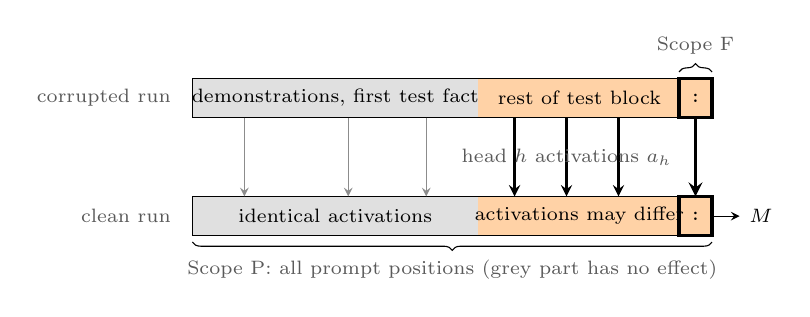
\begin{tikzpicture}[>=stealth, font=\scriptsize]
\def\W{6.6}
% corrupted run
\node[anchor=east, text=black!65] at (-0.15,1.25) {corrupted run};
\fill[black!12] (0,1.0) rectangle (0.55*\W,1.5);
\fill[orange!35] (0.55*\W,1.0) rectangle (\W,1.5);
\draw (0,1.0) rectangle (\W,1.5);
\draw[very thick] (\W-0.42,1.0) rectangle (\W,1.5);
\node at (0.275*\W,1.25) {demonstrations, first test fact};
\node at (0.775*\W-0.2,1.25) {rest of test block};
\node at (\W-0.21,1.25) {\texttt{:}};
% clean run
\node[anchor=east, text=black!65] at (-0.15,-0.25) {clean run};
\fill[black!12] (0,-0.5) rectangle (0.55*\W,0);
\fill[orange!35] (0.55*\W,-0.5) rectangle (\W,0);
\draw (0,-0.5) rectangle (\W,0);
\draw[very thick] (\W-0.42,-0.5) rectangle (\W,0);
\node at (0.275*\W,-0.25) {identical activations};
\node at (0.775*\W-0.2,-0.25) {activations may differ};
\node at (\W-0.21,-0.25) {\texttt{:}};
% arrows: head activations copied
\foreach \x in {0.1,0.3,0.45} {\draw[->, black!45] (\x*\W,1.0) -- (\x*\W,0);}
\foreach \x in {0.62,0.72,0.82} {\draw[->, thick] (\x*\W,1.0) -- (\x*\W,0);}
\draw[->, very thick] (\W-0.21,1.0) -- (\W-0.21,0);
\node[text=black!65] at (0.72*\W,0.5) {head $h$ activations $a_h$};
% braces
\draw[decorate, decoration={brace, amplitude=3pt, mirror}] (0,-0.58) -- (\W,-0.58)
  node[midway, below=3pt, text=black!65] {Scope P: all prompt positions (grey part has no effect)};
\draw[decorate, decoration={brace, amplitude=3pt}] (\W-0.42,1.58) -- (\W,1.58)
  node[midway, above=3pt, text=black!65] {Scope F};
\draw[->] (\W,-0.25) -- ++(0.35,0) node[right] {$M$};
\end{tikzpicture}}
\caption{Single-head activation patching. At a fixed layer, the corrupted run
supplies one head's pre-projection activations to the clean run. Scope~P replaces
all original prompt positions; replacements before the first token difference have
no effect because their activations are identical. Scope~F replaces only the final
colon. The answer contrast is evaluated at the first divergent answer token, leaving
any shared answer prefix unpatched.}
\label{fig:patch}
\end{figure}

\subsection{Characterizing important heads}
\label{sec:method-char}

The causal map says which heads matter and by how much, but not what they do. To
turn a list of heads into hypotheses about a mechanism that Stage~4 can test as
routes and groups, we profile a fixed inventory of 105 heads: every head with a
strong effect on the map, positive or negative, every RI-selected head, a few heads
of moderate effect and the 25 random controls (composition in
Appendix~\ref{app:stage3}). Three questions organize the profile
(Table~\ref{tab:profile}); each is answered per head, and each answer is a
candidate role, not an established one.

\paragraph{Where does the head act?}
Scope-F importance is compared with Scope-P importance, and a single-position scan
patches one test-block position at a time. A head whose effect is confined to the
colon is a candidate \emph{reader}; one whose effect enters at earlier positions is
a candidate \emph{writer}. Neither label follows from the comparison alone: equal
Scope-F and Scope-P effects do not show that the head reads from any particular
position, and single-position effects need not add up to the all-position effect.
Reverse patching, $J_h=M(x_r;\,a_h\leftarrow a^c_h)-M(x_r)$, applies the
intervention in the opposite direction to check its symmetry; recovery is not
assumed and, where found, does not show that one head suffices. The relevance to
the criterion is that the position at which a head's effect enters may differ from
the positions at which it passes the criterion's attention condition or scores
highly on it.

\paragraph{What does it read, and what does it promote?}
At the colon, each head's attention mass is split over the query fact's mother and
child, the distractor mothers and the colon itself, on all prompts rather than only
on events that pass the criterion's gate, so that behaviour the criterion misses is
profiled too. A \emph{changed-query} prompt (the other child is asked about, facts
unchanged) tests whether attention follows the question; reorder and corruption
prompts test whether it follows position. What the head promotes is read from its
actual output vector projected onto the vocabulary, alongside the criterion's
raw-embedding projection of the same position; both are content diagnostics, not
measurements of the effect on the model's output, since a head can act through
later components. Two alternative explanations of a high score are tested directly:
a static preference for repeating tokens (the weight copying score, and whether the
head promotes the name it attends to) and generic induction or retrieval behaviour
(the synthetic probes of \S\ref{sec:rw-readout}). For heads whose effect is
localized to a position that the projections do not explain, a controlled readout
compares the site's residual under the intact head and under a replaced head
activation, with a source-swap control that bounds what the readout can see
(Appendix~\ref{app:stage3}).

\paragraph{What carries the effect?}
At the colon the head's output $A^hV^h$ is recomputed with the attention pattern
$A^h$ and the values $V^h$ taken independently from the clean or the corrupted run.
The two single replacements give a routing term (corrupted pattern, clean values)
and a value term (clean pattern, corrupted values); their sum is compared with the
full patch, and the interaction is reported per family. Whether the values or the
routing dominate is an outcome of this test, not a consequence of the head using
contextual information.

\paragraph{Output of the stage.}
Each head receives a profile: where its effect enters, what it attends to, what its
output promotes, and which alternative explanations apply. The profiles select
components and positions for Stage~4: a head with a localized effect inside a fact
proposes a source position for a route; a later head that attends to that position
proposes a receiver; the routing/value split says which input of the receiver to
test; heads with similar or opposite roles propose groups for redundancy and
interaction tests. Similar profiles are not evidence of a connection. Stage~3
proposes roles and possible connections; Stage~4 tests whether the connections
carry causal effect.

\begin{table}[t]
\centering\small
\setlength{\tabcolsep}{4pt}
\begin{tabular}{@{}p{2.3cm}p{2.5cm}p{2.5cm}@{}}
\toprule
Question & Central test & Use in Stage 4 \\
\midrule
Where does the head act? & Scope F vs.\ P; single-position patches & source and receiver positions \\
What does it read and promote? & query-change control; attention and output profiles & role and connection hypotheses \\
What carries the effect? & attention--value separation & which route input to test \\
\bottomrule
\end{tabular}
\caption{Head profile: questions, central tests and what Stage~4 does with the
answers. Coverage of every measurement is in Appendix~\ref{app:stage3}.}
\label{tab:profile}
\end{table}

\subsection{From heads to a mechanism}
\label{sec:method-circuits}

Stages 2 and 3 measure heads one at a time. The question of the paper is whether
the heads the criterion selects take part in the \emph{mechanism} by which the model
uses a stated relation---heads that pass information to one another, with the
model's MLPs and normalization possibly mediating between them. Stage~3 supplies
the candidates: a localized effect proposes a source position, an attention
profile proposes receivers, and the routing/value split proposes which channel to
test; none of these is yet a connection. Stage~4 asks three questions of them.
All selections use the discovery families; the held-out families are opened once,
for the frozen mechanism.

\paragraph{Communication: which effects between components can be isolated?}
A \emph{route} is a source head, a site, a receiver head and a channel
(Figure~\ref{fig:route}). It is measured in two runs. In a hybrid run, the source's
activation is replaced by its corrupted-run value at the site and the residual
increments of all other components are frozen at their clean values, so that only
the source's change reaches the receiver; the receiver's input on the chosen
channel (keys or values at the site, or its query at the colon) is captured from
this run. In a fresh clean run, the captured channel is injected, only the
receiver's own colon output row changes as a result, and the rest of the model
computes normally to the answer. The change in $M$ is the route effect. A route
shows that the receiver uses what the source wrote, on the declared channel and
against the declared frozen background; it is not an additive share of the
source's total effect, and separately measured routes do not by themselves compose
into a chain. Routes are measured on the 40 common pairs, retained by a fixed
effect-size rule, and the retained ones extended to all 178 pairs in both donor
directions. Sources and receivers come from the Stage-3 profiles and a coverage
check of heads outside the inventory; controls are matched to the type of
intervention (Appendix~\ref{app:stage4}). Where retained routes leave a source's
effect unexplained, a bounded local expansion repeats the measurement with the
MLPs or blocks between source and receiver released rather than frozen; no broad
search over heads is run, and an unresolved source is reported as such.

\paragraph{Joint dependence: how do heads act together, and does a source's
effect need its receivers?}
Retained routes define \emph{groups}: the receivers of one source and the sources
of one receiver. Each group is patched as a whole and minus one member, which gives
the group's nonadditivity $N(S)=I(S)-\sum_{h\in S}I(h)$ and each member's
conditional contribution $\delta_h=I(S)-I(S\setminus\{h\})$. \emph{Receiver
blocking} tests communication in the live model: the source's clean activation is
restored in the corrupted run while its proposed receivers are clamped to their
corrupted outputs; the restoration that is lost measures how much the source's
effect depends on the receivers' response (with self-clamp and reverse controls).
Because of interactions and overlapping paths it is not a partition of the source's
effect into shares. \emph{RI participation} tests the RI-selected heads that pass a
fixed relevance rule (31 heads): each is measured alone, in the intact model and on
a weakened background in which a strong reader has been replaced so that a masked
contribution can show, and the residual RI heads (the 23 without a strong
standalone effect) are compared as a group with layer-matched cohorts of
non-selected heads of the same size. A \emph{backup} test applies the same logic
to a head that moves names strongly but has a negligible standalone effect.
Selected group contrasts are repeated with mean-activation replacement in place of
the corrupted donor, since the baseline changes the strength of group effects.

\paragraph{Explanation quality: does a reduced set of heads preserve the behaviour
and its dependence on facts and query?}
A candidate set $C_0$ is fixed by rule from the strong heads, the coverage
candidates and the RI heads that pass the conditional test. In the \emph{retained}
model (Figure~\ref{fig:retained}) the heads of $C$ stay live at all test-block
positions and the output of every \emph{other head} at those positions is replaced
by its role-matched mean; embeddings, MLPs, normalization, demonstrations and the
answer prefix stay live, so the claim is a head mechanism conditional on the rest
of the model. $C$ is accepted if, family by family, it preserves the model's
clean-minus-corrupted gap, its candidate accuracy in each condition and each order,
and does so more than an all-heads-mean baseline (thresholds in
Appendix~\ref{app:stage4}). The accepted set is \emph{reduced} by removing
pre-declared blocks of heads while the guards hold, and its \emph{completeness} is
checked by removing the same blocks from the full model and from the reduced set
and comparing the losses. Finally, a four-cell panel crosses the fact swap with a
\emph{query change}, with the answer sign held fixed across all four cells, so that
the interaction
\begin{equation}
\label{eq:bd}
B_D=\tfrac14\,\mathbb{E}_{f,o}\!\left[M_D(x_{00})-M_D(x_{10})-M_D(x_{01})+M_D(x_{11})\right]
\end{equation}
measures whether a configuration's answer preference follows the queried binding
rather than the fact swap alone; the
preference and accuracy in each cell are reported alongside it, since a mean
interaction can hide a failing cell. The panel is run on the full model, on the
full model minus the main receiver group and minus the residual RI group, on the
reduced set $C^*$, and on $C^*$ minus its RI members or minus its non-RI members.
The last two test collective dependence on RI-selected heads \emph{inside} the
retained mechanism; they do not show that each member has a relational role or
that the criterion identifies it uniquely. The mask, rosters and thresholds are
frozen before the held-out families are evaluated.

\begin{figure}[t]
\centering
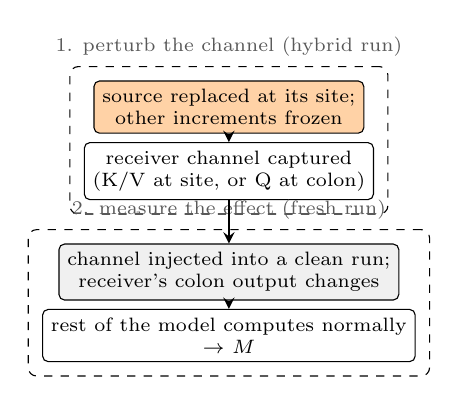
\begin{tikzpicture}[>=stealth, font=\scriptsize, node distance=3pt,
  box/.style={draw, rounded corners=2pt, inner sep=3pt, align=center, minimum width=3.3cm},
  zone/.style={draw, dashed, rounded corners=3pt, inner sep=5pt},
  lab/.style={text=black!65}]
\node[box, fill=orange!35] (S) at (0,0) {source replaced at its site;\\other increments frozen};
\node[box, below=of S] (C) {receiver channel captured\\(K/V at site, or Q at colon)};
\node[zone, fit=(S)(C), label={[lab]above:1. perturb the channel (hybrid run)}] (Z1) {};
\node[box, fill=black!6, below=0.55cm of C] (I) {channel injected into a clean run;\\receiver's colon output changes};
\node[box, below=of I] (M) {rest of the model computes normally\\$\rightarrow$ $M$};
\node[zone, fit=(I)(M), label={[lab]above:2. measure the effect (fresh run)}] (Z2) {};
\draw[->, thick] (S) -- (C);
\draw[->, thick] (C) -- (I);
\draw[->, thick] (I) -- (M);
\end{tikzpicture}
\caption{A route. Zone 1: the source is replaced and all other residual increments
are frozen, so the receiver's channel reflects only the source's change. Zone 2:
the captured channel is injected into a fresh clean run; the receiver's colon output
changes and the rest of the model runs normally to the answer.}
\label{fig:route}
\end{figure}

\begin{figure}[t]
\centering
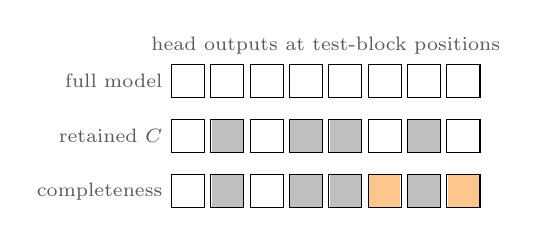
\begin{tikzpicture}[>=stealth, font=\scriptsize,
  head/.style={draw, minimum width=0.42cm, minimum height=0.42cm, inner sep=0pt},
  lab/.style={text=black!65}]
\foreach \r/\name in {0/full model, 1/retained $C$, 2/completeness} {
  \node[lab, anchor=east] at (-0.2,-\r*0.7) {\name};
  \foreach \i in {0,...,7} {\node[head] (h\r\i) at (\i*0.5,-\r*0.7) {};}
}
\foreach \i in {1,3,4,6} {\fill[black!25] ([shift={(-0.2,-0.2)}]h1\i.center) rectangle ++(0.4,0.4);}
\foreach \i in {1,3,4,6} {\fill[black!25] ([shift={(-0.2,-0.2)}]h2\i.center) rectangle ++(0.4,0.4);}
\foreach \i in {5,7} {\fill[orange!45] ([shift={(-0.2,-0.2)}]h2\i.center) rectangle ++(0.4,0.4);}
\node[lab] at (1.75,0.45) {head outputs at test-block positions};
\end{tikzpicture}
\caption{The retained-mechanism test. Only head outputs at test-block positions are
intervened on. White: head live. Grey: head output replaced by its role-matched
mean. Orange: a block removed for the completeness check, removed identically from
the full model. MLPs, normalization, embeddings, demonstrations and the answer
prefix are live in every configuration.}
\label{fig:retained}
\end{figure}

\subsection{Developmental check}
\label{sec:method-dev}

The second gap of \S\ref{sec:sih} concerns training: \citet{ren2024semantic} infer
that SIHs drive the emergence of in-context learning from the co-timing of a
behavioural transition with rising indices in heads selected because their index
rises. We run an adapted version of that analysis on OLMo-2's public pre-training
checkpoints: not a replication of the original emergence point, which a different
model, training run and preprocessing can shift, but a test of the same
developmental relation inside our model.

\paragraph{Design.}
Behaviour is measured as in the original, with the same four synthetic
classification task families, the same shot ladder and the same distinction
between format compliance and pattern discovery; accuracy is constrained to the
legal task labels, and format validity is checked separately against the
vocabulary-wide top token. Fifty frozen prompts per task and shot count are reused
at every checkpoint (17 checkpoints, 1B--3.9T tokens), so comparisons are paired.
The relation index is computed for all 1,024 heads at ten of these checkpoints on
700 balanced AGENDA relation triplets, with the original developmental gate (source
token is the attention argmax) as primary and the full $\tau{=}2.2$ gate as
sensitivity. Two additions go beyond the original. First, alongside the index over
gated events, we record how often the gate passes and the index per measurement
opportunity, in which events that fail the gate contribute zero; a developmental
change can then be located in routing frequency or in selectivity among routed
events. Second, instead of following selected rising curves, the heads with the
highest index at the final checkpoint are traced backwards and the overlap between
each checkpoint's top heads and the final set is measured, which tests whether the
early and the mature high-index heads are the same heads. The broad behavioural
window was fixed before the index timing was analysed; three checkpoints inside it
were added to the behavioural measurement after a routing peak had been seen in the
index, and the results keep the two apart (Appendix~\ref{app:dev}).

\section{Results}
\label{sec:results}

We report the four audit stages in the order of \S\ref{sec:method}.
Results use discovery data; aggregation, per-head estimates and sensitivity
analyses are detailed in Appendices~\ref{app:stage1}--\ref{app:stage4}.

\subsection{RI poorly identifies causal contributors}
\label{sec:results-why}

\paragraph{What RI selects.}
Under the descriptive percentile rule, the published pooled index selects two
heads whose qualifying attention is exclusively self- or previous-token
attention. Demonstrations contribute over 99\% of their summed scores
(Table~\ref{tab:pooled}), consistent with static token preferences rather
than evidence of retrieval. A separate matched-target test finds no head with
a significant preference after Holm correction; neither pooled-index head
has eligible matched events. The descriptive test-only rule selects
59 heads, with several candidates sensitive to the current token,
target anchor or fact order (Appendix~\ref{app:stage1}).

\begin{figure}[t]
\centering
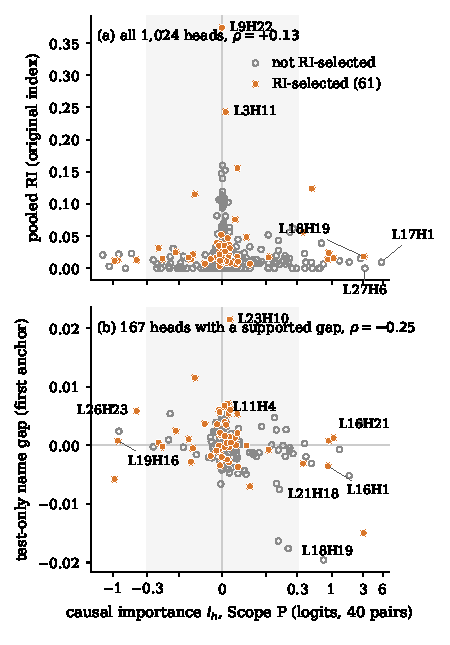
\includegraphics[width=\columnwidth]{fig_ri_vs_importance}
\caption{RI versus signed causal importance (Scope~P, exact patching,
40 common pairs; symmetric-log axis). Orange: the combined 61-head
selection. (a) Pooled RI for all heads. (b) First-token name gap for
167 supported heads. Shading marks $|I_h|<0.3$.}
\label{fig:ri-vs-imp}
\end{figure}

\paragraph{Against the causal map.}
Pooled RI correlates weakly with signed importance ($\rho=0.13$),
while the test-only name gap correlates negatively
($\rho=-0.25$, and $-0.30$ within layer; Figure~\ref{fig:ri-vs-imp}).
The two pooled-index heads have near-zero measured effects.
Of the combined 61 selected heads, 48 have $|I_h|<0.1$,
less than 1\% of the clean--corrupted gap.
Among the 148 heads measured on all 178 pairs, 25 have
$|I_h|\geq0.3$, but only eight are selected.
The test-only selection also misses 88 of the 102 heads with the
largest positive common-subset effects.
Both selections are incomplete; the pooled selection additionally
meets our pre-registered misleading criterion
(Appendix~\ref{app:stage2}).

\paragraph{Why RI can miss retrieval.}
At the answer position, the current token is always a colon:
with unchanged visible token IDs, raw-embedding RI cannot adapt
its name preferences when mothers are reassigned.
All 49 jointly qualifying L16H21 clean/corrupted query pairs
exhibit this invariance.
A further hypothesis is that copying a current non-target name
raises the name-control score, penalizing potentially useful heads;
\S\ref{sec:results-char} examines this explanation.
These limitations concern the index, not the model's capacity
for semantic computation.

\subsection{The causal map}
\label{sec:results-map}

\paragraph{A few heads carry most of the effect.}
The gradient screen reproduces the exact ranking (Spearman 0.945 on the same
pairs), so the map below rests on exact patching wherever it is reported
(Appendix~\ref{app:stage2}). Against a mean clean--corrupted gap of 11.2 logits,
replacing a single head moves the metric by up to 5.7 logits (L17H1, half of the
gap), and three further heads each move it by about a quarter; all four have the
expected sign in every family (Figure~\ref{fig:causal-map}a). Twenty-five heads
reach $|I_h|\ge0.3$: 17 positive and 8 negative, the latter moving the model
\emph{toward} the stated fact when their corrupted-run output is inserted. Effects
of this size are not independent shares of the gap, since single-head patches can
interact. The same four heads lead the exact all-head scan on the common subset,
with effects within 5\% of their 178-pair values, so the leading heads are not an
artefact of the extension set (Appendix~\ref{app:stage2}).

\begin{figure}[t]
\centering
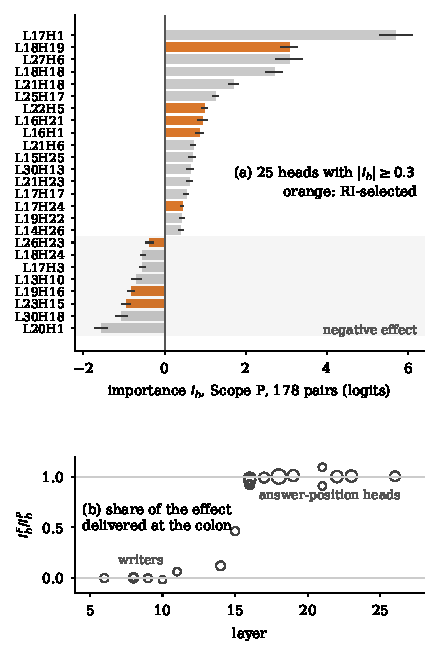
\includegraphics[width=\columnwidth]{fig_causal_map}
\caption{The causal map. (a) Signed Scope-P importance of the 25 strong heads on
all 178 pairs, with family-bootstrap intervals; orange marks RI-selected heads.
(b) Ratio of Scope-F to Scope-P importance by layer for the 20 heads of the
Scope-F set with $|I_h|>0.04$; marker size grows with $|I_h|$.}
\label{fig:causal-map}
\end{figure}

\paragraph{Two positions, two kinds of head.}
Restricting the patch to the final colon splits the map by depth
(Figure~\ref{fig:causal-map}b). Every measurable head in layers 16--26 keeps
between 91\% and 109\% of its effect when only the colon is patched, so its
contribution is delivered at the answer position; every measurable head in layers
6--11 loses all of it, so it acts only through what it writes at earlier test
positions for later components to read; two heads in layers 14--15 are
intermediate. The stored logits show how the
answer-position heads act: the positive ones raise the logit of the name retrieved
on the donor run and leave the alternative almost untouched, and the negative ones
lower it (Table~\ref{tab:scopeF-app}). The sign alone does not say by what
mechanism---promotion of an attended name, suppression of it, or an indirect
path---and the three strongest heads lie outside this Scope-F set;
\S\ref{sec:results-char} localizes every strong head's effect and tests these readings.

These positional differences suggest a writer--reader organization, but do not
identify computations or connections. The next stages characterize the heads
(\S\ref{sec:results-char}) and test causal routes between them
(\S\ref{sec:results-routes}).

\subsection{What the important heads do}
\label{sec:results-char}

\paragraph{Where the heads act, and what the writer writes.}
Twenty of the 25 strong heads deliver their whole effect at the colon
($I^F_h/I_h$ between 0.96 and 1.07; Appendix~\ref{app:stage3}). The exception is
the strongest head: L17H1 has no effect at the colon and acts inside the query
fact, at the mother's tokens, at ``is'' and at the period
(Figure~\ref{fig:profiles}a). At ``is'', ``of'' and the period the two prompts
have identical inputs, so the head's output there depends on the preceding mother
and matters for the answer. L15H25 acts at the last token of the query child. The
main writer thus sits in the same layer band as the readers, and the shallow heads
of \S\ref{sec:results-map} are all weak. A controlled readout of the residual at
``is'' exposes a mother-token preference that depends on L17H1: replacing the head
shifts the readout by $-0.46$ against $-0.52$ for the full source swap, negative in
all 20 families. This supports an identity-sensitive write, not a relational
binding; the content at L15H25's site is unresolved, since the readout does not
respond even to the source swap.

\begin{figure}[t]
\centering
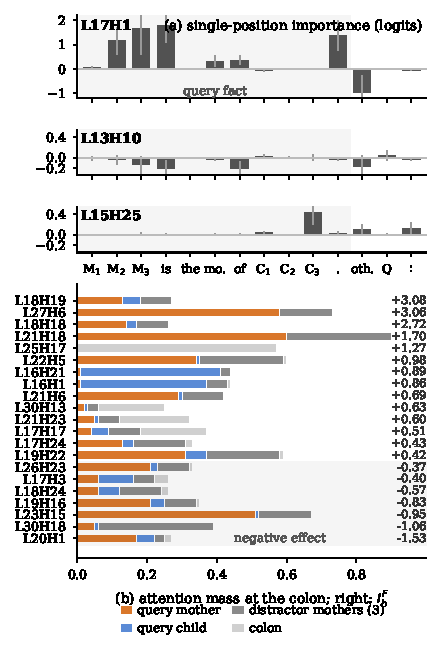
\includegraphics[width=\columnwidth]{fig_head_profiles}
\caption{Head profiles. (a) Single-position patches of the three fact-position
heads, summed by token role in the query fact (M: mother tokens, C: child tokens,
oth.: the other test facts, Q: question, colon); family mean and SD over the 20
common families. (b) Attention mass at the colon of the strong answer-position
heads, split over the query mother, the query child, the three distractor mothers
and the colon itself, with each head's Scope-F importance.}
\label{fig:profiles}
\end{figure}

\paragraph{What the readers select and what they carry.}
The answer-position heads fall into three attention types
(Figure~\ref{fig:profiles}b): mother-attenders, of both signs; child-attenders,
which select the second mention of the queried child; and heads whose largest
target is the colon itself. For the mother- and child-attenders, changing only the
question moves attention to the newly queried fact in all 20 common families
(controls: at most a fifth of that shift), while reordering or swapping the mothers
leaves the family-mean attention almost unchanged. One negative head, L30H18,
attends to the distractor mothers. Separating attention from values at the colon,
value replacement carries most of the mean effect for the leading heads (L18H19:
values $+3.16$, pattern $+0.08$): the source selection follows the question, and
the swap acts through what is read there. Family-level interactions are large,
however, so separability is not assumed downstream. What the heads write is only
partly visible in their output vectors: L27H6 writes the answer directly ($+3.0$
logits for the query mother over the distractors), but for L18H19, L18H18, the
strong negative heads and the child-attenders the projection is far below the
effect. Their causal effects are not explained by this projection, which motivates
tests of downstream mediation. Recomputing the criterion from each head's actual
contextual input does not repair its correlation with importance ($-0.26\to-0.17$
on the 68 supported heads).

\paragraph{Copying is part of the story, not the mechanism.}
Six heads promote the first token of the name they attend to in at least 80\% of
events and one suppresses it; at the last-token anchor every label disappears. For
the positive movers the RI name gap is negative precisely at events whose current
token is a control name, as the copy-penalizing account of \S\ref{sec:results-why}
predicts. But copying is neither necessary nor sufficient (Appendix~\ref{app:stage3}):
the strongest weight copier hurts the answer by copying the distractor, and L23H15
favours the name it attends to while its effect is $-0.95$, so the sign of a head's
projection is not the sign of its effect. ``Negative mover'' covers at least two
patterns, and how L23H15 acts is open.

The profiles turn the map into testable connections: a fact-position writer whose
sites may feed the mother-attenders' keys or values, a second writer at the child
for the child-attenders, strong colon heads whose effects need a downstream path,
and positive and negative movers whose joint behaviour is untested
(\S\ref{sec:results-routes}).

% \input{sections/06_discussion}

% Placeholder labels for results subsections not yet written; remove when they exist.
\subsection{Routes and groups}\label{sec:results-routes} TODO.
\subsection{Emergence is not identity}\label{sec:results-dev} TODO.

\section*{Limitations}
TODO.

\section*{AI Disclosure and Reflection}
TODO (required by the course guidelines).

% Working list of papers from the project's papers/ folder that the text cites.
% Update whenever a new paper from that folder is used. Each line: local file name -> bib key -> link.
% This section is a writing aid; decide before submission whether to keep it (e.g. as
% "Sources consulted") or remove it. It is placed just before \bibliography in main.tex.

\section*{Papers used (working list)}
\begin{itemize}\setlength\itemsep{0pt}\small
\item \texttt{Identifying Semantic Induction Heads to Understand In-Context Learning.pdf}
  --- \texttt{ren2024semantic} ---
  \href{https://arxiv.org/abs/2402.13055}{arXiv:2402.13055} (cited in \S\ref{sec:sih}, App.~\ref{app:ri})
\item \texttt{In-context Learning and induction heads.pdf}
  --- \texttt{olsson2022induction} ---
  \href{https://transformer-circuits.pub/2022/in-context-learning-and-induction-heads/index.html}{Transformer Circuits, 2022}
  (cited in \S\ref{sec:sih}, App.~\ref{app:ih})
\item (not in folder) A Mathematical Framework for Transformer Circuits
  --- \texttt{elhage2021mathematical} ---
  \href{https://transformer-circuits.pub/2021/framework/index.html}{Transformer Circuits, 2021}
  (cited in \S\ref{sec:sih}, App.~\ref{app:ri}, App.~\ref{app:ih})
\item \texttt{Retrieval Head Mechanistically Explains.pdf}
  --- \texttt{wu2024retrieval} ---
  \href{https://arxiv.org/abs/2404.15574}{arXiv:2404.15574} (cited in \S\ref{sec:sih}, App.~\ref{app:ih})
\item \texttt{The Evolution of Statistical Induction Heads.pdf}
  --- \texttt{edelman2024evolution} ---
  \href{https://arxiv.org/abs/2402.11004}{arXiv:2402.11004} (cited in App.~\ref{app:ih})
\item \texttt{interpretability in the wild a circuit in gpt2 small.pdf}
  --- \texttt{wang2023ioi} ---
  \href{https://arxiv.org/abs/2211.00593}{arXiv:2211.00593} (cited in \S\ref{sec:rw-patching}, \S\ref{sec:rw-readout}, \S\ref{sec:rw-circuits})
\item \texttt{how to activation patching.pdf}
  --- \texttt{heimersheim2024patching} ---
  \href{https://arxiv.org/abs/2404.15255}{arXiv:2404.15255} (cited in \S\ref{sec:rw-patching})
\item \texttt{TOWARDS BEST PRACTICES OF ACTIVATION PATCHING IN LANGUAGE MODELS - METRICS AND METHODS.pdf}
  --- \texttt{zhang2024bestpractices} ---
  \href{https://arxiv.org/abs/2309.16042}{arXiv:2309.16042} (cited in \S\ref{sec:rw-patching})
\item \texttt{Patchscopes.pdf}
  --- \texttt{ghandeharioun2024patchscopes} ---
  \href{https://arxiv.org/abs/2401.06102}{arXiv:2401.06102} (cited in \S\ref{sec:rw-readout})
\item \texttt{Towards Automated Circuit Discovery.pdf}
  --- \texttt{conmy2023acdc} ---
  \href{https://arxiv.org/abs/2304.14997}{arXiv:2304.14997} (cited in \S\ref{sec:rw-circuits})
\item \texttt{Position-aware Automatic Circuit Discovery.pdf}
  --- \texttt{haklay2025position} ---
  \href{https://arxiv.org/abs/2502.04577}{arXiv:2502.04577} (cited in \S\ref{sec:rw-circuits})
\item \texttt{Have Faith in Faithfulness Going Beyond Circuit Overlap.pdf}
  --- \texttt{hanna2024faithfulness} ---
  \href{https://arxiv.org/abs/2403.17806}{arXiv:2403.17806} (cited in \S\ref{sec:rw-circuits})
\item (not in folder) Attribution Patching Outperforms Automated Circuit Discovery
  --- \texttt{syed2023attribution} ---
  \href{https://arxiv.org/abs/2310.10348}{arXiv:2310.10348} (cited in \S\ref{sec:method-causal})
\end{itemize}


\bibliography{refs}

\appendix
\section{The relation index of \citet{ren2024semantic}}
\label{app:ri}

This appendix restates the SIH criterion as defined in the original paper (their
\S3, Eq.~2--3), so that the main text can stay short, and lists the evidence behind
the limitations noted in \S\ref{sec:sih}. Our own re-implementation, with its
controls and calibration, is described in \S\ref{sec:method-ri}.

\paragraph{Notation.}
The model has $L$ layers of $H$ heads. For head $h$, $W^h_{OV}=W^h_v W^h_o$ is the OV
matrix, $W^h_{QK}=W^h_q (W^h_k)^{\top}$ the QK matrix, $W_e$ the input embedding and
$W_U$ the unembedding. For an input $[t_1,\ldots,t_n]$, $x_i=t_i W_e$ is the
\emph{input embedding} of token $t_i$. A relation is a triplet $T=(t_s,r,t_o)$ with
head token at position $s$ and tail token at position $o$.

\paragraph{Step 1: attention condition (QK).}
At a current position $j\ge\max(s,o)$, let $A^h_j$ be head $h$'s attention over
positions $1..j$, written in the original paper as $\mathrm{softmax}(x_j W^h_{QK}
x^{\top}/\sqrt{d_h})$ in the notation of Eq.~1 there. The head qualifies for $(T,j)$
if
\begin{equation*}
s=\arg\max_{k\le j} A^h_{j,k}
\quad\text{and}\quad
\frac{A^h_{j,s}}{\max_{k\ne s} A^h_{j,k}}>\tau,\qquad \tau=2.2 .
\end{equation*}
The paper's formula writes the attention in terms of the embedding matrix $x$; in our
implementation $A^h_j$ is the attention pattern actually produced by the model's
forward pass at the head's layer (captured from the attention kernel), and only the
OV projection of Step~2 uses the raw embedding.

\paragraph{Step 2: output condition (OV).}
The head's output at $j$ is projected onto the vocabulary from the input embedding of
the current token,
\begin{equation*}
p^{h,j}=\mathrm{softmax}\!\left(x_j W^h_{OV} W_U\right)\in\mathbb{R}^{|V|}.
\end{equation*}
Only the tokens $t_k$, $k\le j$, that appear in the context are kept (duplicates
counted once). Their probabilities are centred and clipped,
$q^{h,j}_{t_k}=\max\!\big(0,\;p^{h,j}_{t_k}-\mathbb{E}_{k'\le j}[p^{h,j}_{t_{k'}}]\big)$,
and the score for $(T,j)$ is the share of the clipped mass on the tail token,
\begin{equation*}
a^{h,j}_T=\frac{q^{h,j}_{t_o}}{\sum_{k\le j} q^{h,j}_{t_k}} .
\end{equation*}

\paragraph{Worked example.}
Table~\ref{tab:ri-example} carries the computation through for one event, with
illustrative numbers. The context is ``Anna is the mother of Ben .'' and the current
token is the period ($j{=}7$), so seven distinct tokens are visible. Suppose head $h$
attends most to \emph{Anna} with a margin above $\tau$, so the event qualifies with
$t_s{=}$Anna. The raw-embedding projection of the period is pushed through $W^h_{OV}W_U$
and the softmax is restricted to the visible tokens; the mean of the seven values,
$\bar p{=}0.143$, is subtracted and negatives are clipped. The tail token \emph{Ben}
holds $0.52$ of the clipped mass, which is the event score. Two properties of the
score are visible here: it depends only on the current token's embedding and on
which tokens are visible, so every event of this head at a period with the same
visible set receives the same vector $p$; and the tail competes with all visible
tokens, including \emph{is} and \emph{the}, not with other names.

\begin{table}[h]
\centering\scriptsize
\setlength{\tabcolsep}{2pt}
\begin{tabular}{@{}lrrrrrrr@{}}
\toprule
$t_k$ & Anna & is & the & mother & of & Ben & . \\
\midrule
$p^{h,j}_{t_k}$ & 0.30 & 0.05 & 0.05 & 0.15 & 0.05 & 0.32 & 0.08 \\
$q^{h,j}_{t_k}$ & 0.157 & 0 & 0 & 0.007 & 0 & 0.177 & 0 \\
\bottomrule
\end{tabular}
\caption{Illustrative event score. $q=\max(0,p-\bar p)$ with $\bar p=0.143$;
$\sum_k q_k=0.341$; $a^{h,j}_T=q_{\text{Ben}}/\sum_k q_k=0.177/0.341=0.52$. The numbers are chosen for
the example, not measured.}
\label{tab:ri-example}
\end{table}

\paragraph{Step 3: aggregation.}
$\mathrm{RI}_h$ is the mean of $a^{h,j}_T$ over all qualifying $(T,j)$ for a given
relation type. There is no threshold that turns an index into a label: the paper
reports heatmaps of $\mathrm{RI}_h$ per relation and calls heads with salient values
SIHs. An appendix of the original paper shows that $\tau\in\{2.0,2.5\}$ yields a
similar set of salient heads.

\paragraph{Setting of the original study.}
InternLM2-1.8B (24 layers, 16 heads); the AGENDA test set (1,000 abstracts with
annotated knowledge graphs); three syntactic dependencies (subject, object,
modifier) and seven relation types; multi-token entities replaced by single capital
letters and frequent function words removed before scoring.

\paragraph{Evidence for the limitations in \S\ref{sec:sih}.}
\begin{itemize}\setlength\itemsep{1pt}
\item[(i)] The word ``ablation'' occurs once in the original paper and refers to
varying $\tau$ (their Appendix~A). No activation, weight or attention intervention is
reported.
\item[(ii)] The training analysis (their \S4.2) uses a model the authors train
themselves ($d{=}2048$, 40k steps on SlimPajama, checkpoints every 200 steps), not
the released InternLM2-1.8B in which the SIHs of \S3 are identified. In that analysis
the margin condition on $\tau$ is dropped (``it is too challenging to find attention
heads having an extremely high attention probability''), and the plotted heads are
``sampled \ldots with an increasing relation index''. The inference is stated as
``we infer that the formation of semantic induction heads plays a crucial role in the
development of the ICL ability.''
\item[(iii)] The projection $x_j W^h_{OV} W_U$ uses $x_j=t_j W_e$. The paper justifies
this by quoting \citet{elhage2021mathematical}: ``both the QK circuit and OV circuit
are directly performed on input embeddings.'' That statement describes attention-only
models without MLPs and normalization, where the residual at every layer is a sum of
head outputs added to the embedding; in a 24- or 32-layer model with MLPs and
layer normalization the value input of head $h$ at position $j$ is the normalized
residual $\mathrm{LN}(r^{\ell}_j)$, and the head's output at $j$ is
$\sum_k A^h_{j,k}\,\mathrm{LN}(r^{\ell}_k)W^h_{OV}$, a function of the attended
positions $k$.
\item[(iv)] In $a^{h,j}_T$ the tail competes with every earlier distinct token, not
with tokens of the same type (other entities), and no reference distribution for
$\mathrm{RI}_h$ is reported.
\end{itemize}

\section{Induction heads: background}
\label{app:ih}

\citet{elhage2021mathematical} decompose an attention head into a query--key (QK)
circuit, which decides where the head attends, and an output--value (OV) circuit,
which decides what the head writes. In one- and two-layer attention-only models they
identify \emph{induction heads}: on a sequence $[A][B]\ldots[A]$, the QK circuit
attends from the second $[A]$ to $[B]$ (prefix matching) and the OV circuit raises the
logit of $[B]$ (copying). \citet{olsson2022induction} define both properties
behaviourally, as a prefix-matching score and a copying score measured on repeated
random token sequences, and show that ablating induction heads removes most of the
in-context loss reduction of small models; they also observe that induction heads form
in a narrow window of training that coincides with a sharp improvement in in-context
learning.

\begin{figure}[h]
\centering
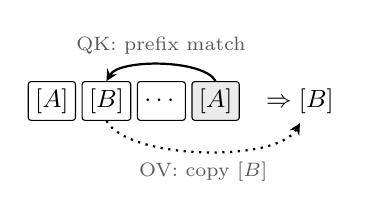
\begin{tikzpicture}[tok/.style={draw, rounded corners=1pt, minimum height=1.4em, inner sep=2.5pt, font=\small},
  lab/.style={font=\scriptsize, text=black!65}, >=stealth, node distance=2pt]
\node[tok] (a1) {$[A]$}; \node[tok, right=of a1] (b1) {$[B]$}; \node[tok, right=of b1] (d) {$\cdots$};
\node[tok, right=of d, fill=black!8] (a2) {$[A]$}; \node[right=6pt of a2, font=\small] (out) {$\Rightarrow [B]$};
\draw[->, thick] (a2.north) to[out=120, in=60, looseness=0.6] node[lab, above, pos=.5] {QK: prefix match} (b1.north);
\draw[->, thick, dotted] (b1.south) to[out=-60, in=-120, looseness=0.6] node[lab, below, pos=.5] {OV: copy $[B]$} (out.south);
\end{tikzpicture}
\caption{The induction-head template. The QK circuit attends from the second $[A]$
to the token that followed the first, and the OV circuit raises that token's logit.
The SIH criterion keeps the template but lets the written token differ from the
attended one: it attends to $t_s$ and writes $t_o$ (Figure~\ref{fig:ri}).}
\label{fig:ih}
\end{figure}

Two later developments are relevant here. \citet{wu2024retrieval} identify
\emph{retrieval heads}, heads with the same behavioural signature that copy a needle
from a long context; they show that a small set of such heads is largely universal
across models and that masking them destroys long-context factual recall, whereas
masking random heads does not. \citet{edelman2024evolution} study how statistical
induction heads emerge during training on Markov-chain data and show that in-context
learning develops through phases in which simpler statistical strategies precede the
induction mechanism.

Two features of this literature are the contrast for semantic induction heads. First,
the head type is defined by a behaviour the head produces on a controlled input, so a
head either performs the behaviour or does not. Second, the importance of the head
type is established by intervention on the model, not by the score alone. In our
setting the repeated-sequence and key--value retrieval probes of
\S\ref{sec:method-char} apply these behavioural tests to every head in our inventory.

\section{Compute, runs and released artifacts}
\label{app:compute}

All GPU work ran on the Tel Aviv University Slurm cluster (partition
\texttt{studentkillable}) on TODO-GPU-TYPE GPUs of 11--12\,GB memory each; the model
is sharded in fp16 over two GPUs per worker. Table~\ref{tab:compute} lists the
production runs. Every run is driven by a frozen plan whose SHA-256, together with
the hashes of the code files and the model revision, is written to a manifest; a
gate at the start of each run reproduces reference candidate logits and, where
applicable, previously saved importances to a fixed tolerance before any
measurement, and the run aborts otherwise. Records carry per-item provenance and
runs resume from checkpoints. Code, plans, manifests and analysis tables are at
\url{https://github.com/Maxgolu/NLP_proj}.

\begin{figure}[h]
\centering
\resizebox{\columnwidth}{!}{%
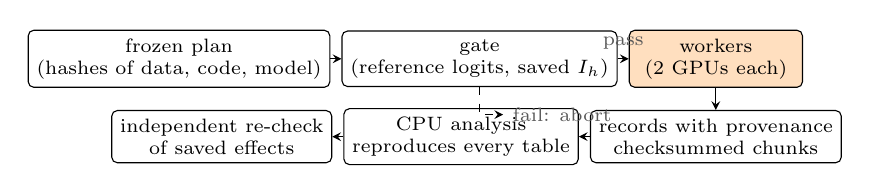
\begin{tikzpicture}[>=stealth, font=\scriptsize, node distance=4pt,
  box/.style={draw, rounded corners=2pt, inner sep=3pt, align=center, minimum width=2.2cm, minimum height=1.6em}]
\node[box] (plan) {frozen plan\\(hashes of data, code, model)};
\node[box, right=of plan] (gate) {gate\\(reference logits, saved $I_h$)};
\node[box, right=of gate, fill=orange!25] (run) {workers\\(2 GPUs each)};
\node[box, below=8pt of run] (rec) {records with provenance\\checksummed chunks};
\node[box, left=of rec] (ana) {CPU analysis\\reproduces every table};
\node[box, left=of ana] (ver) {independent re-check\\of saved effects};
\draw[->] (plan) -- (gate); \draw[->] (gate) -- node[above, text=black!65] {pass} (run);
\draw[->] (run) -- (rec); \draw[->] (rec) -- (ana); \draw[->] (ana) -- (ver);
\draw[->, dashed] (gate.south) |- ++(0.3,-0.35) node[right, text=black!65] {fail: abort};
\end{tikzpicture}}
\caption{Run protocol shared by every stage. A run starts from a frozen plan, passes a
gate that reproduces reference quantities, writes checksummed records, and its
analysis tables are recomputed on CPU from those records and re-checked
independently.}
\label{fig:pipeline}
\end{figure}

\begin{table}[h]
\centering\scriptsize
\setlength{\tabcolsep}{3pt}
\begin{tabular}{@{}llrp{2.5cm}@{}}
\toprule
Run & Job & Wall-clock & Content \\
\midrule
Stage 1, RI scan & TODO & TODO & all 1,024 heads, 534 prompts \\
Stage 1, test-only RI & 905839 & TODO & name/word controls \\
Stage 2, causal map & 888691 & 1h15m (6 GPUs) & all heads, 40 pairs; 92 heads, 178 pairs \\
Stage 2, extension & 912879 & 33m & Scope P/F, 178 pairs \\
Stage 3, characterization & TODO & $\approx$3.7h (6 GPUs) & 263,328 patched forwards \\
Stage 3, readout & 918689 & 33m & 1,920 readout records \\
Stage 4, routes and groups & TODO & TODO & TODO \\
Developmental sweep & TODO & TODO & 17 checkpoints \\
\bottomrule
\end{tabular}
\caption{Production runs. Wall-clock is the Slurm elapsed time of the job.}
\label{tab:compute}
\end{table}

\section{Prompt format and variants}
\label{app:data}

Figure~\ref{fig:data} shows the test block of one discovery family in its variants.
Every prompt begins with four demonstrations of the same form (four facts, a
question and its answer), identical across all variants and orders of a family, so
that twins differ only in the test block. A test block holds two chains of two facts
each: the \emph{query chain}, whose middle name is asked about, and a
\emph{distractor chain} of the same shape. The answer is the mother of the queried
name, i.e.\ the top of the query chain; the distractor is the top of the other chain.
The queried name therefore occurs three times (as a mother, as a child, and in the
question), and the two candidate answers occur once each. All names are generated
strings absent from the model's vocabulary as single tokens; names are
length-matched under the OLMo-2 tokenizer so that clean and corrupted prompts are
aligned position by position. Relation annotations (head, tail, character spans) are
produced at construction time for every fact, including demonstrations.

\begin{figure*}[t]
\centering\scriptsize
\setlength{\tabcolsep}{8pt}
\begin{tabular}{@{}p{0.48\textwidth}p{0.48\textwidth}@{}}
\toprule
\textbf{Clean} (answer: Rarnia) & \textbf{Corrupted} (answer: Dirlna) \\
\midrule
\texttt{Jarlia is the mother of Kernna.} & \texttt{Jarlia is the mother of Kernna.} \\
\texttt{\textbf{Rarnia} is the mother of Jarlia.} & \texttt{\textbf{Dirlna} is the mother of Jarlia.} \\
\texttt{Kulnra is the mother of Tilnia.} & \texttt{Kulnra is the mother of Tilnia.} \\
\texttt{\textbf{Dirlna} is the mother of Kulnra.} & \texttt{\textbf{Rarnia} is the mother of Kulnra.} \\
\texttt{Question: Who is the mother of Jarlia?} & \texttt{Question: Who is the mother of Jarlia?} \\
\texttt{Answer:} & \texttt{Answer:} \\
\midrule
\textbf{Reorder} (answer: Rarnia) & \textbf{Other fact order} (answer: Rarnia) \\
\midrule
\texttt{Kulnra is the mother of Tilnia.} & \texttt{Kulnra is the mother of Tilnia.} \\
\texttt{Jarlia is the mother of Kernna.} & \texttt{Dirlna is the mother of Kulnra.} \\
\texttt{Rarnia is the mother of Jarlia.} & \texttt{Jarlia is the mother of Kernna.} \\
\texttt{Dirlna is the mother of Kulnra.} & \texttt{Rarnia is the mother of Jarlia.} \\
\texttt{Question: Who is the mother of Jarlia?} & \texttt{Question: Who is the mother of Jarlia?} \\
\texttt{Answer:} & \texttt{Answer:} \\
\bottomrule
\end{tabular}
\caption{Test block of discovery family 0 (the four demonstrations that precede it
are omitted). Top: the clean prompt and its corrupted twin; only the two bold names
are swapped, so the two prompts are token-aligned and the distractor becomes the
answer. Bottom left: the reorder variant, with the same facts in a different order.
Bottom right: the second fact order of the clean prompt, in which the distractor
chain precedes the query chain. The query fact is the one whose child is the queried
name (``Rarnia is the mother of Jarlia.''); the final colon of ``Answer:'' is the
answer position at which Scope-F interventions are applied.}
\label{fig:data}
\end{figure*}


\begin{table}[h]
\centering\scriptsize
\begin{tabular}{@{}lr@{}}
\toprule
Quantity & Value \\
\midrule
Generated families & 200 \\
4-shot accuracy, clean / corrupted / reorder (both orders) & 93 / 94 / 89\% \\
Families correct on clean and corrupted, both orders & 176 \\
\quad discovery / held-out (split by family id) & 89 / 87 \\
Clean--corrupted pairs, discovery & 178 \\
Common subset (all-head measurements) & 20 families / 40 pairs \\
Prompts per family (base, corrupted, reorder $\times$ 2 orders) & 6 \\
Demonstrations per prompt & 4 \\
Prompt length, tokens (mean) & 282 \\
Positions differing between twins (mean) & 44 \\
Pairs with a shared answer prefix & 4 \\
\bottomrule
\end{tabular}
\caption{Data set and split.}
\label{tab:data}
\end{table}

\section{Relation-index scan: details and sensitivity}
\label{app:stage1}

\paragraph{Run.}
The scan (\texttt{stage1\_v4\_calibrated}) covered all 1,024 heads on 534 prompts
(89 discovery families $\times$ base/corrupted/reorder $\times$ two orders, four
demonstrations each). Preflight checks reproduced the behavioural candidate scores
and showed zero drift under inert hooks and self-patching; attention capture had a
maximum vocabulary-logit drift of 0.039 on one prompt. The test-only extension
(\texttt{ri\_test\_v2}) scored all 46,634 saved test-block events; 237,685
replication checks of saved scores passed. Independent recomputation reproduced all
reported means, contrasts and support counts.

\paragraph{Method details.}
\emph{Event score.} For a qualifying $(T,j)$ with anchor token $t_o$, the score is
$a^{h,j}_T=q^{h,j}_{t_o}/\sum_{k\le j}q^{h,j}_{t_k}$ with
$q^{h,j}_t=\max(0,p^{h,j}_t-\bar p^{h,j})$ and
$p^{h,j}=\mathrm{softmax}(x_jW^h_{OV}W_U)$ restricted to the distinct token ids
visible at $j$ (Appendix~\ref{app:ri}); anchor-token collisions between target and
control names are treated as ties. \emph{Aggregation.} Scores are averaged within
family and then with equal weight across the families that have at least one
scored event for that head; families without events do not enter the mean.
\emph{Name controls.} The other test-fact mothers whose full name is visible at
$j$; token length need not match. \emph{Word controls.} Up to three word types
sampled from the visible non-name tokens of the prompt (mostly template words);
they provide a weaker specificity check. All reported means and counts use the
name-control-eligible subset of events; events without an available control are
excluded from the gap statistics but retained in the pooled index.
\emph{Calibration population.} Test-block events in which both the target and a
control mention are fully visible, of equal token length and with distinct first
tokens; 19,901 of 278,134 QK events qualify. Heads need at least 50 such events
across ten families (80 heads). The null swaps target and control labels
consistently within each family (100{,}000 replicates) and assumes the two labels
are exchangeable under the null; heads are tested with Holm correction over 1,024.
\emph{Selection population.} All name-control-eligible events; a ranking requires
at least 20 events in ten families. The 50-event threshold of the calibration and
the 20-event threshold of the selection are different requirements for different
purposes and yield different head populations.

\paragraph{Why the pooled index is dominated by demonstrations.}
Under the original pooled index and the descriptive 99.9th-percentile rule the two
top heads are L3H11 and L9H22. Table~\ref{tab:pooled} splits their events by block:
demonstrations contribute over 99\% of each head's summed target score, and neither
head has a single event from a test position attending to a demonstration source.
Inspection of the events shows why: all 86 passes of L9H22 attend from a position to
itself, and all 149 passes of L3H11 attend one token back, from a period or newline
to the end of the preceding name. In both cases the OV projection is computed from
the same current-token embedding for every event, so the reported index varies only
with which target token is selected and how the visible context normalizes it. A
high pooled index can thus be obtained from local attention with a static token
preference, without any event that demonstrates retrieval of a test relation. This
does not show that these heads take no part in relational retrieval; it shows that
the pooled score does not require it, which motivates the test-block restriction of
\S\ref{sec:method-ri}.

\begin{table}[h]
\centering\scriptsize
\setlength{\tabcolsep}{3pt}
\begin{tabular}{@{}lrrrr@{}}
\toprule
Head & Pooled RI & QK freq.\ (\%) & Demo: $n$ / RI & Test: $n$ / RI \\
\midrule
L3H11 & 0.243 & 0.0097 & 144 / 0.250 & 5 / 0.038 \\
L9H22 & 0.374 & 0.0056 & 72 / 0.445 & 14 / 0.007 \\
\bottomrule
\end{tabular}
\caption{The two heads selected by the pooled index and the descriptive
99.9th-percentile rule, split by whether the annotated fact and the current position
lie in a demonstration or in the test block. Frequency is the share of eligible
fact--position evaluations that pass the QK gate.}
\label{tab:pooled}
\end{table}

\paragraph{Matched-target calibration.}
The matched subset retained 19,901 of 278,134 QK events; 80 heads had at least 50
matched events across ten families. Under 100{,}000 family-consistent target/control
swaps, no head passed Holm correction at $\alpha{=}0.05$, over 1,024 or over the 80
supported heads. The three smallest raw $p$ values are L16H4 ($p{=}0.006$, target
0.0147 vs.\ control 0.0093, 87 events, 40 families), L9H18 ($p{=}0.023$) and L13H13
($p{=}0.025$). Neither pooled-index head had a matched event.

\paragraph{Test-only candidates.}
Table~\ref{tab:ricands} lists the leading heads under the test-only index with name
controls (all test facts, all test positions). The frozen rule (\S\ref{sec:method-ri})
selects 59 heads in total, 36 of which enter at least one name-gap ranking. Two
patterns recur among high scorers. Some heads owe much of their score to events in
which the current token is part of the target name itself (L23H10: 31 of 60
comparisons; L15H18: 104 of 110); such events can be scored without any retrieval
across positions, so they do not demonstrate it, although they do not exclude it.
Excluding those events reduces but does not remove L23H10's gap. Others depend on one current token (for L17H5 the
token \emph{mother} contributes 66\% of the family-weighted target score) or on the
reorder variant (299 of L9H16's 343 comparisons). Paired base/corrupted events
that follow the changed fact are rare: L11H4 has 21 jointly passing pairs in 18
families, with a positive name gap in both versions for only five families.

\begin{table}[h]
\centering\scriptsize
\setlength{\tabcolsep}{3pt}
\begin{tabular}{@{}llrrrrr@{}}
\toprule
Head & Anchor & Events & Fam. & Target & Control & Gap \\
\midrule
L11H4  & first & 94  & 39 & 0.0147 & 0.0081 & $+0.0065$ \\
L17H5  & first & 65  & 34 & 0.0229 & 0.0168 & $+0.0061$ \\
L9H16  & last  & 343 & 87 & 0.0209 & 0.0135 & $+0.0074$ \\
L12H2  & first & 52  & 32 & 0.0201 & 0.0129 & $+0.0072$ \\
L25H18 & last  & 46  & 17 & 0.0287 & 0.0156 & $+0.0131$ \\
L23H10 & first & 60  & 24 & 0.0283 & 0.0068 & $+0.0215$ \\
\bottomrule
\end{tabular}
\caption{Leading test-only candidates (all test facts and positions). Events are
target/control comparisons; family-weighted means over the name-control-eligible
subset.}
\label{tab:ricands}
\end{table}

\paragraph{The answer position and the raw-embedding invariance.}
At the final colon, 20 heads have qualifying events (748 in total, 744 to test
sources); L16H21 and L16H1 attend to the query fact in over 220 prompts each (41\%
of prompts). Their name gaps at that position are near zero or negative
(Table~\ref{tab:final}). Part of the reason is structural. The current token at the answer position is
always the colon, so for a fixed head the raw-embedding projection vector is the same
in every prompt, and the normalized score is the same whenever the set of visible
token ids is the same; only the attention condition can differ between such prompts.
In all 49 jointly passing base/corrupted pairs of L16H21 the sign of the
old-versus-new-mother contrast flips exactly when the target label flips, at both
anchors: once the head attends, the scoring component cannot follow a reassignment
of mothers at this position. The same holds at any earlier position whose current
token and visible token set are unchanged. This is a limit of the score, not a
statement about what the head's actual output carries.

\begin{table}[h]
\centering\small
\begin{tabular}{@{}lrrrrr@{}}
\toprule
Head & Query events & Fam. & QK (\%) & First gap & Last gap \\
\midrule
L16H21 & 222 & 77 & 41.6 & $-0.0004$ & $+0.0034$ \\
L16H1  & 223 & 76 & 41.8 & $-0.0025$ & $-0.0034$ \\
L16H24 & 68  & 35 & 12.7 & $-0.0028$ & $+0.0036$ \\
L16H4  & 63  & 32 & 11.8 & $+0.0004$ & $-0.0072$ \\
\bottomrule
\end{tabular}
\caption{Heads whose attention at the answer position selects the query fact
(denominator 534 prompts), with their name gaps at the two anchors.}
\label{tab:final}
\end{table}

\begin{figure}[h]
\centering
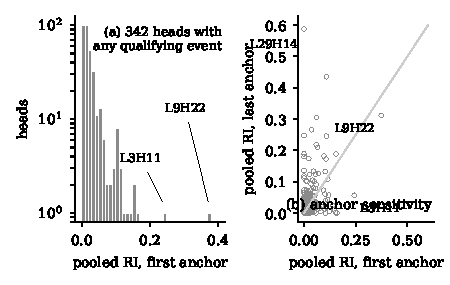
\includegraphics[width=\columnwidth]{figE_ri_distribution}
\caption{The pooled index over heads. (a) Distribution of the first-anchor index for
the 342 heads with at least one qualifying event (log count); the two heads selected by
the percentile rule are marked. (b) First- against last-anchor index for all heads;
the anchor changes which heads lead (L29H14 tops the last-anchor ranking).}
\label{fig:ri-dist}
\end{figure}

\paragraph{Dominance margin.}
Over all 1,455,940 eligible dominance ratios (event-weighted, demonstrations
included), 80.9\% are at or below the published $\tau{=}2.2$ and the 95th percentile
is 4.48. Refiltering the saved passes at 4.48 keeps 72,797 events; the two pooled
heads keep 30 and 49 passes respectively. The anchor also matters: under the last
token, L29H14 tops the conditional-strength ranking (Figure~\ref{fig:ri-dist}b). All such variants are reported
as sensitivity analyses; the audit itself keeps the published parameters.

\section{Causal map: details}
\label{app:stage2}

\paragraph{Coverage and head sets.}
The screen was computed for all heads on all 178 discovery pairs. Exact Scope-P
patching covered all 1,024 heads on a common subset of 20 randomly chosen families
(40 pairs). Exact Scope-P patching on all 178 pairs covered 148 heads: a 92-head set
selected on discovery data before the extension measurements (the screen's top 25,
the two heads selected by the original pooled index, fixed Stage-1 example heads
and 25 random controls), the 46 test-only RI candidates not already in that set, and
ten further heads completing the set of 19 heads with at least one answer-position
QK event to a test-fact source. Exact Scope-F patching on all 178 pairs covered the
union of the 59 RI candidates and the 19 answer-position heads (69 heads). The
extension heads were chosen after the common-subset results were available and
before any measurement on the remaining 138 pairs; their selection uses discovery
data only, so intervals for selected heads describe stability within the run and
are not selection-adjusted. Twenty-five heads with the largest common-subset effects
were all already covered, since the 92-head set contained the screen's top 25. The
common-subset values of the extension heads were taken from the existing all-head
run, not recomputed; a reproduction check on six heads of one family matched the
saved effects exactly.

\paragraph{Gates.}
Before measurement, each worker verified zero drift of the behavioural candidate
scores under hooks, zero effect of self-patching (at all positions and at the final
position), zero self-attribution, and zero effect of patching positions before the
first differing token, whose activations are identical under causal attention.

\paragraph{Screen calibration.}
On the 40 common pairs, with the same pairs for both, the signed head-ranking
Spearman correlation between $\widehat I_h$ and exact $I_h$ is 0.945 (0.921 for
absolute means, 0.903 pair-by-head), above the pre-registered 0.7, so the
integrated-gradients fallback was not used. Among the 148 extension heads on the
identical 178 pairs the correlation is 0.990; comparing the 178-pair screen with the
40-pair exact values gives 0.698, a difference that mixes approximation error with
family sampling. Rank agreement does not imply per-head accuracy: the screen
under-shoots the strongest heads (same-pair residuals L17H1 2.24, L27H6 0.51,
L18H19 0.28 logits), as expected of a local linear approximation.

\begin{figure}[h]
\centering
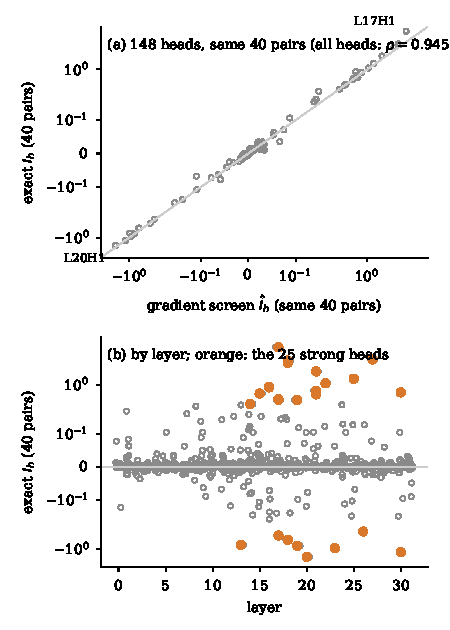
\includegraphics[width=\columnwidth]{figF_screen_layers}
\caption{The causal map. (a) Gradient screen against exact importance on the same 40
pairs for the 148 heads with full coverage (symmetric-log axes); the screen
under-shoots the strongest head. (b) Exact importance of all 1,024 heads by layer;
orange marks the 25 heads with $|I_h|\ge0.3$ on the 178 pairs. Strong heads of both
signs lie in layers 13--30.}
\label{fig:map-app}
\end{figure}

\paragraph{Behavioural contrast.}
Over the 89 discovery families (orders averaged) the clean metric is 5.68
[5.34, 6.03], the corrupted metric with the clean sign fixed $-5.49$
[$-5.85$, $-5.14$], and the gap 11.17 [10.63, 11.73]; every clean pair has $M>0$ and
every corrupted pair $M<0$. Four of the 178 pairs have a non-empty shared answer
prefix. Intervals are percentile family bootstraps (20,000 resamples), computed
after the results were seen.

\paragraph{Stability across subsets and orders.}
The all-head exact scan on the 20-family common subset ranks the same four heads
first, with effects 5.742 (L17H1), 3.222 (L27H6), 3.080 (L18H19) and 2.768
(L18H18) against 5.701, 3.071, 3.072 and 2.704 on all 178 pairs.
Over all 1,024 heads the Spearman correlation between the order-0 and order-1
exact rankings on the common subset is 0.46, a value dominated by the many heads
with near-zero effect; within the 92-head extension set it is 0.73 and among the
top 25 it is 0.66, with 17 heads in both order-specific top-25 lists. All ten
strongest heads have positive mean importance in both orders.

\paragraph{Scope F: how the answer-position heads act.}
Table~\ref{tab:scopeF-app} splits the Scope-F effect of the strongest heads of the
69-head Scope-F set into the change of the clean-answer, corrupted-answer and
source-name logits at the first divergent token. For the 69 heads the two scopes
correlate at 0.79, but the ratio $I^F_h/I^P_h$ is bimodal: between 0.91 and 1.09 for
every head in layers 16--26 with $|I_h|>0.04$, indistinguishable from zero for every
such head in layers 6--11 (L6H24, L8H8, L8H15, L9H16, L10H16, L11H15), and
intermediate for L14H23 (0.12) and L15H3 (0.46). The promotion is not perfectly
specific to the answer: for L18H19, L16H21 and L16H1 the logit of the source (child)
name also rises by 0.3--0.4, so a Scope-F effect shows that the head raises the name
retrieved on the donor run, not that it retrieves only the correct one.

\begin{table}[h]
\centering\scriptsize
\setlength{\tabcolsep}{3pt}
\begin{tabular}{@{}lrrrrr@{}}
\toprule
Head & $I^P_h$ & $I^F_h$ & $\Delta$ clean & $\Delta$ corr. & $\Delta$ source \\
\midrule
L18H19 & 3.07 & 3.08 & $-0.20$ & $+2.88$ & $+0.37$ \\
L22H5  & 0.98 & 0.98 & $-0.06$ & $+0.92$ & $+0.02$ \\
L16H21 & 0.93 & 0.89 & $+0.01$ & $+0.90$ & $+0.32$ \\
L16H1  & 0.87 & 0.86 & $-0.05$ & $+0.81$ & $+0.33$ \\
L17H24 & 0.43 & 0.43 & $-0.03$ & $+0.40$ & $+0.06$ \\
L26H23 & $-0.37$ & $-0.37$ & $+0.08$ & $-0.29$ & $-0.06$ \\
L19H16 & $-0.82$ & $-0.83$ & $0.00$ & $-0.83$ & $-0.16$ \\
L23H15 & $-0.95$ & $-0.95$ & $+0.01$ & $-0.94$ & $-0.19$ \\
\bottomrule
\end{tabular}
\caption{Scope-F patch of the eight strongest heads in the Scope-F set: importance
under both scopes and the mean change of the clean-answer, corrupted-answer and
source (child) name logits, 89 families, orders averaged. Positive heads promote the
name retrieved on the donor run rather than suppressing the alternative; negative
heads lower it.}
\label{tab:scopeF-app}
\end{table}

\paragraph{Pre-registered audit criteria.}
The selection is judged \emph{sound} if selected heads have systematically larger
importance than layer-matched non-selected heads; \emph{incomplete} if heads in the
top decile of exact importance lie outside the selection, with the reason recorded
(no qualifying QK event, insufficient support, or a supported but non-positive name
gap at both anchors); and \emph{misleading} if the median importance of selected
heads does not exceed that of the 25 random controls (family bootstrap of the median
difference). The criteria are not mutually exclusive. They were written for the
pooled index and re-applied to the test-only selection, whose membership was
decided after Stage-1 results were inspected; the second application is
exploratory.

\paragraph{Rank correlations and verdicts.}
Table~\ref{tab:corr-app} lists the Spearman correlations between the Stage-1
statistics and exact importance on the 40 common pairs; support means at least 20
comparisons in ten families. The two pooled-index heads have $I_h=-0.002$ logits on
all 178 pairs, with the expected sign in 47\% and 42\% of families, against a median
of 0.0002 for the 25 random controls. Top-25 overlap with the exact ranking is 0.02
by Jaccard for both RI versions, against 0.52 for the gradient screen. Of the 102
heads in the top decile of importance, 88 lie outside the test-only selection: 23
have no qualifying attention event, 22 fall below the support rule, 18 pass with a
non-positive name gap at both anchors, and 25 have a positive gap that did not reach
any top ten. The two strongest misses illustrate two of these routes: L17H1
($I_h=5.70$) has only two qualifying attention events in the whole scan, and L27H6
($I_h=3.07$) has 85 qualifying events but a pooled index of zero, so its
raw-embedding projection does not favour the target at those events. Under the pre-registered criteria the pooled index is
\emph{incomplete} (101 of the 102 top-decile heads fall below even the lenient
control threshold of 0.137; the second-strongest head has index zero) and
\emph{misleading} (median importance of its two heads $-0.0021$ against 0.0002 for
the random controls); soundness is not supported. Re-applied to the test-only
selection: incomplete (88 of 102 top-decile heads outside it); the median importance
of selected heads exceeds the controls by 0.003 logits (bootstrap interval
[0.0009, 0.0067]), 0.03\% of the gap, with 56\% positive signs against 60\% for the
controls; the pooled layer-matched difference is $+0.035$ logits [0.023, 0.047] but
positive in only 12 of 28 layers and carried by four heads in layers 16--22 that the
gradient screen had already selected.

\begin{table}[h]
\centering\scriptsize
\setlength{\tabcolsep}{3pt}
\begin{tabular}{@{}lrr@{}}
\toprule
Statistic & $n$ & $\rho$ vs.\ $I_h$ \\
\midrule
Pooled index, first anchor (all heads) & 1,024 & $+0.135$ \\
Test-only target, first anchor & 172 & $-0.013$ \\
Test-only name gap, first anchor & 167 & $-0.252$ \\
\quad ranks within layer & 158 & $-0.302$ \\
\quad without layers 16--18 & 144 & $-0.278$ \\
\quad without the 25 strongest heads & 153 & $-0.214$ \\
\quad positive gaps only & 78 & $-0.102$ \\
\quad self-attention events only & 39 & $-0.537$ \\
Test-only name gap, query fact, first & 103 & $-0.335$ \\
Test-only name gap, last anchor & 167 & $-0.091$ \\
Control-name mean (other visible names) & 167 & $+0.143$ \\
Gradient screen (Eq.~\ref{eq:screen}) & 1,024 & $+0.945$ \\
\bottomrule
\end{tabular}
\caption{Spearman rank correlations with exact Scope-P importance on the 40 common
pairs. Family-bootstrap interval for the main name-gap value: $[-0.289,-0.169]$.}
\label{tab:corr-app}
\end{table}

\section{Head characterization: details}
\label{app:stage3}

\paragraph{Inventory.}
The 105 heads comprise: 48 RI-selected heads with small causal effect; 12 strong
positive heads outside the RI selection; 5 strong positive RI-selected heads; 8
strong negative heads; 7 moderate heads ($0.1\le|I_h|<0.3$); and the 25 random
controls of the causal map. ``RI-selected'' here means the 59 test-only candidates
plus the two heads of the original pooled index (61 heads). ``Strong'' means
$|I_h|\ge0.3$ logits on the 178-pair Scope-P mean; the thresholds were applied
within the 148 heads that have full exact coverage, so heads outside that set are
not thereby shown to be weak. Membership (Table~\ref{tab:inventory}) was fixed from the saved causal map before
any Stage-3 measurement. Each run began with a gate that reproduced saved Stage-2
effects on probe heads, verified that the reconstructed attention patterns match the
model's attention output within tolerance, and verified that the joint
attention+value replacement equals the ordinary head patch.

\begin{table}[h]
\centering\scriptsize
\setlength{\tabcolsep}{3pt}
\begin{tabular}{@{}p{2.3cm}p{5.0cm}@{}}
\toprule
Group ($n$) & Heads \\
\midrule
Strong positive, not RI-selected (12) & L14H26, L15H25, L17H1, L17H17, L18H18, L19H22, L21H6, L21H18, L21H23, L25H17, L27H6, L30H13 \\
Strong positive, RI-selected (5) & L16H1, L16H21, L17H24, L18H19, L22H5 \\
Strong negative (8) & L13H10, L17H3, L18H24, L19H16, L20H1, L23H15, L26H23, L30H18 \\
Moderate ($0.1\le|I_h|<0.3$) (7) & L6H24, L7H1, L8H15, L12H17, L14H23, L15H3, L16H31 \\
RI-selected, small effect (48) & L1H27, L2H21, L2H22, L3H11, L4H0, L5H18, L6H2, L7H18, L7H25, L8H8, L8H16, L9H6, L9H16, L9H17, L9H22, L10H16, L11H3, L11H4, L11H7, L11H15, L12H2, L12H9, L13H1, L13H22, L14H10, L15H0, L15H2, L15H18, L15H28, L15H29, L16H2, L16H4, L16H16, L16H24, L17H5, L18H15, L20H7, L20H14, L21H24, L21H25, L21H27, L23H10, L24H17, L25H18, L26H31, L27H23, L30H3, L31H1 \\
Random controls (25) & L0H1, L2H1, L6H12, L9H23, L9H26, L11H20, L11H27, L13H30, L15H27, L18H5, L18H22, L19H20, L21H11, L21H22, L22H15, L22H31, L23H17, L25H11, L25H13, L25H15, L25H20, L25H21, L28H1, L28H15, L29H5 \\
\bottomrule
\end{tabular}
\caption{The 105-head inventory, fixed from the saved causal map before any Stage-3
measurement.}
\label{tab:inventory}
\end{table}

\begin{table}[h]
\centering\scriptsize
\setlength{\tabcolsep}{3pt}
\begin{tabular}{@{}lll@{}}
\toprule
Measurement & Heads & Inputs \\
\midrule
Scope F vs.\ P, promotion/suppression & 105 & 178 pairs \\
Single-position scan & 105 & 40 pairs \\
Reverse patching & top 10 $|I_h|$ & 178 pairs \\
Attention profile + controls & 105 & 20 fam.\ $\times$ 8 prompts \\
Output projections & 105 & 20 families, colon \\
Attention--value separation & 105 & 178 pairs \\
Weight copying score & 105 & 314 name-token ids \\
Attended-name contrast & 105 & 160 prompts \\
Matched contextual RI & 70 & saved Stage-1 events \\
Synthetic probes & 105 & 992 + 32 probes \\
Controlled readout & 2 & 4 sites, 40 pairs \\
\bottomrule
\end{tabular}
\caption{Coverage of the Stage-3 measurements.}
\label{tab:stage3cov}
\end{table}

\paragraph{Single-position scan and reverse patching.}
For each common pair and inventory head, the corrupted activation is inserted at
one test-block position at a time, from the first differing token to the colon;
query-fact positions are labelled (mother tokens, ``is'', ``of'', child tokens,
period). Reverse patching inserts the clean activation into the corrupted run for
the ten heads with the largest $|I_h|$, at Scope P and Scope F, to test the
intervention in the opposite direction and its symmetry.

\paragraph{Attention profile and controls.}
On the 20 common families, both orders, four prompt types are captured: base,
corrupted, reorder and changed-query. Attention at the colon is summed over the
token spans of the query mother, the query child, each distractor mother and the
colon, for every head on every prompt, independently of the criterion's gate.
Controls are paired within family. Family means and per-prompt absolute changes are
both reported, since signed means can hide opposite-sign changes.

\paragraph{Output projections.}
The contextual projection is $o^h_jW_U$ with $o^h_j$ the head's actual output
vector at the colon (before the shared post-attention normalization of OLMo-2,
which is not assigned to heads); the contrast is the query mother's first-token
logit minus the mean over the distractor mothers' first tokens. The raw-embedding
projection uses $x_jW^h_{OV}W_U$ with $x_j$ the colon's embedding, as in the
criterion. Both are diagnostics of one vector, not attributions of the causal
effect.

\paragraph{Attention--value separation.}
For each pair, the head's output at the colon is recomputed as $A^hV^h$ with the
pattern and the values taken independently from the clean or the corrupted run;
the reconstruction is gated against the actual attention output. The interaction is
the full patch minus the sum of the two single replacements, reported as a family
mean and as a mean absolute value.

\paragraph{Weight copying and attended-name contrast.}
The weight score projects each of the 314 first/last test-name token ids through
$W^h_{OV}W_U$ and takes the token's own logit minus the mean over the other token
ids in the set; a 128-token ordinary-word sample serves as reference. The
attended-name contrast uses every test-block event of the 160 core prompts in
which the head's attention argmax lies inside a visible test name: the contextual
logit of that name's first token minus the mean over the other visible distinct
names. Classification rule, fixed in advance, with four outcomes: with at least 20
events in ten families, \emph{name mover} if the contrast is positive in
$\ge80\%$ of events, \emph{negative name mover} if negative in $\ge80\%$, and
\emph{neither} otherwise; with fewer events or families, \emph{insufficient}.
Variants: last-token anchor, same-role controls, non-self events, colon-site events,
base prompts only.

\paragraph{Matched contextual RI.}
For every saved Stage-1 event of an inventory head, the raw embedding in the OV
projection is replaced by the head's actual normalized value input at the same
position, with events, controls, anchors and family weights unchanged; 70 heads
have valid events. This isolates the embedding choice from every other ingredient
of the criterion.

\paragraph{Synthetic probes.}
Repeated random token sequences and key--value retrieval contexts are presented to
the model; for each head, attention to the copy source (argmax rate) and the sign of
its output on the gold token are recorded. The model's accuracy on the probes is
reported with the results.

\paragraph{Controlled readout.}
For the two heads whose effect localizes to positions inside the query fact and is
not explained by the output projections, the residual after the head's block is
captured at those positions on the 40 common pairs and injected at a placeholder in
one of two readout prompts at the same layer: an identity completion (``cat $\to$
cat; \ldots; x $\to$'') and a prompt that asks for the mother of the injected entity
(``Fact about a person: x. Question: Who is the mother of this person? Answer:'').
Conditions: intact clean source; source with the head's activation replaced by its
corrupted-run value at the site; the same replacement from the first differing token
to the site; intact corrupted source; the same token role in the other answer-side
fact; no injection. The statistic is $C=\log p(t_q)-\log p(t_o)$ for the first
tokens of the query mother and the other candidate, with paired shifts from the
intact condition. The source-swap condition is essential: if the readout does not
respond to the full entity swap, a null head effect is uninformative. A gate
verified that injecting a prompt's own residual leaves the readout unchanged and
that a self patch leaves the residual unchanged. Head dependence is read only from
the intact-versus-replaced contrast of a multi-component residual.

\paragraph{Results: where the effect enters.}
Of the 25 strong heads, 20 have $I^F_h/I_h\in[0.96,1.07]$, with $I^F_h$ of the
expected sign in $\ge97.8\%$ of families for every strong positive head and
$\le4.5\%$ for every strong negative head. The five others: L17H1 ($I_h=+5.70$,
$I^F_h=-0.06$), L15H25 ($+0.68$, $+0.17$), L14H26 ($+0.40$, $+0.01$; diffuse over
template words), L13H10 ($-0.68$, $-0.03$) and L17H3 ($-0.55$, $-0.40$; mixed).
Random controls have $|I^F_h|\le0.019$ except L18H22 ($+0.089$, equal to its Scope-P
effect). Reverse patching of the ten largest heads recovers the metric by close to the
noising effect at both scopes (L17H1 $+5.21$ vs.\ 5.70; L18H19 $+3.22$ vs.\ 3.07;
L27H6 $+3.06$; L18H18 $+2.85$; L21H18 $+1.75$; L25H17 $+1.27$; L22H5 $+1.01$; L20H1
$-1.63$; L30H18 $-1.20$; L23H15 $-0.93$); recovery is conditional on the rest of the
corrupted model. Single-position sums track the all-position effect in the aggregate
(Spearman 0.91 over 105 heads) but with large cancelling residuals for L17H1 (mean
absolute residual per family 0.89 logits, maximum 2.33), so the profile is not an
additive partition. L13H10 mirrors L17H1 with the opposite sign (``is'' $-0.22$, ``of'' $-0.22$, mother last $-0.14$). L17H1's family-mean effects by role: mother tokens $+0.05/+1.15/
+1.67$, ``is'' $+1.77$, ``mother'' $+0.33$, ``of'' $+0.36$, child $\approx0$, period
$+1.38$, other facts $-0.96$ in total, question and colon $\approx0$. The Scope-F
effect of every strong colon head is dominated by the corrupted-answer logit (88--98\%
of $I^F_h$); L27H6 alone also lowers the clean answer ($+1.96$ and $+1.10$).

\paragraph{Results: attention and output.}
Mother-attenders (mass on the query mother): L27H6 0.58, L21H18 0.60, L23H15 0.51,
L22H5 0.34, L19H22 0.31, L21H6 0.30, L19H16 0.21, L26H23 0.21, L20H1 0.17, L18H18
0.14, L18H19 0.13, L17H24 0.13. Child-attenders: L16H21 0.40, L16H1 0.36. Self-attenders:
L25H17 0.57, L13H10 0.42, L21H23 0.20, L30H13 0.19, L17H17 0.19. Random controls:
mean 0.017 on the query mother. Under a changed query the shift toward the newly
queried fact is positive in 20 of 20 families for every mother- and child-attender
(L21H18 $+1.07$, L23H15 $+0.91$, L27H6 $+0.84$, L16H21 $+0.83$, L16H1 $+0.68$;
controls $\le+0.18$); L30H18 moves away ($-0.19$). Reordering and corruption change
the family-mean mass on the query mother by at most 0.11 and 0.085, but per-prompt
absolute changes reach 0.49 (L21H18), so invariance holds on average only; the model
answers 38 of the 40 changed-query prompts. Contextual projection (query mother minus
distractor mothers, first token): L27H6 $+2.99$, L30H13 $+0.76$, L22H5 $+0.41$,
L21H6 $+0.33$, L21H18 $+0.25$, L30H18 $-0.88$; L18H19 $+0.16$, L18H18 $+0.11$,
L25H17 $+0.16$, L20H1 $-0.09$, L23H15 $+0.04$, L19H16 $-0.04$, L16H21 and L16H1
within $\pm0.02$. Raw-embedding projection: all within $\pm0.008$ (Spearman with
$I^F_h$ $-0.07$). Matched contextual RI (70 heads with valid events): Spearman of the
main name gap with importance $-0.26\to-0.17$; the raw target statistic $+0.01\to
+0.02$. Weight copying score: Spearman $+0.37$ with signed $I_h$, $+0.02$ with
$|I_h|$; L30H18 $+0.60$, L21H6 $+0.35$, L26H23 $-0.20$, L27H6 $+0.04$, L18H18
$-0.08$, L17H1 $+0.01$. Current-token partition of the saved RI events: for L18H19,
L21H18 and L21H6 the name gap is $-0.023$, $-0.017$ and $-0.025$ when the current
token is a control name and within $\pm0.004$ otherwise.

\begin{figure}[h]
\centering
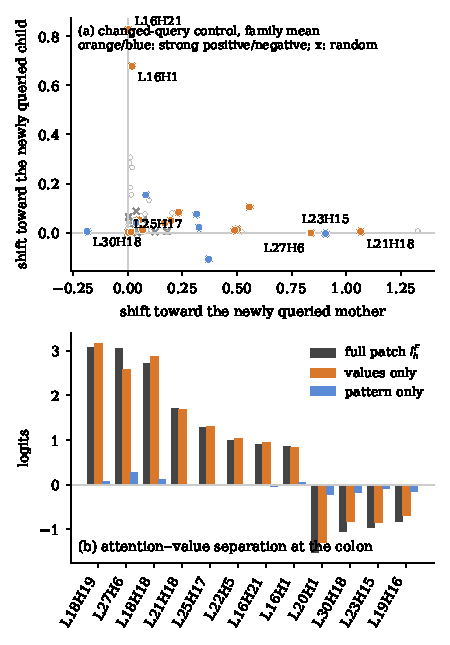
\includegraphics[width=\columnwidth]{figG_attention_values}
\caption{(a) Changed-query control: family-mean shift of attention toward the newly
queried mother ($x$) and child ($y$) for all 105 heads. Mother-attenders move along
$x$, child-attenders along $y$, random controls (crosses) barely move; L30H18 moves
away. (b) Attention--value separation at the colon for the twelve strongest
answer-position heads: the ordinary Scope-F patch beside the values-only and
pattern-only replacements (178 pairs).}
\label{fig:stage3-app}
\end{figure}

\paragraph{Results: attended-name labels and fingerprints.}
Name movers: L27H6 (96\% of 768 events), L17H24 (94\%), L26H31 (91\%), L18H19
(84\%), L22H5 (82\%), L21H6 (82\%); negative name mover: L20H1 (17\% positive).
L21H18 (79\%), L19H22 (78\%), L19H16 (77\% negative) and L26H23 (79\% negative) miss
the rule; L23H15 favours the attended name in 64\% of 2,428 events; L30H18 in 67\%
(mean $+0.60$) while attending to the distractor. L18H19's label rests on earlier-site
events (its colon-site subset is insufficient). L26H31 puts 0.09 of its colon mass on
the query mother and selects the answer in 13\% of its colon-site name events. On the
synthetic probes (model accuracy 100\% and 96\%), retrieval-type attention is shown by
L19H16 (0.97), L21H18 (0.88), L23H15 (0.84), L18H18 (0.56), L16H1 (0.47) and
induction-type attention by L23H15 (0.66), L21H6 (0.64), L16H1 (0.45); L19H16,
L26H23 and L23H15 attend to the source without promoting it. L27H6, L17H1, L20H1 and
L30H18 show no fingerprint. Copying is neither necessary nor sufficient for a strong
effect: L18H18 ($I_h=2.70$) and L27H6 are not copiers by weight ($-0.08$, $+0.04$);
L30H18, the strongest weight copier ($+0.60$), attends to the distractor and hurts
the answer; L26H31 promotes the attended name as strongly as L27H6 (mean contrast
$+2.09$) but rarely attends to the answer and has $I^F_h=+0.027$.

\paragraph{Results: attention--value separation and readout.}
Values: L18H19 $+3.16$ (pattern $+0.08$), L27H6 $+2.59$ ($+0.27$), L18H18 $+2.88$
($+0.11$), L21H18 $+1.70$ ($+0.01$), L25H17 $+1.29$ ($-0.02$); routing terms for the
negative heads L20H1 $-0.22$, L30H18 $-0.18$, L19H16 $-0.16$. Mean absolute
family-level interaction: 1.25 logits for L27H6 (maximum 4.58), 0.81 for L18H18, 0.54
for L18H19. Readout (Table~\ref{tab:readout-app}): at L17H1/``is'' the identity
contrast falls from $+0.515$ to $+0.056$ after head replacement ($-0.006$ for the
corrupted source, $+0.002$ for the other-fact control), negative in every family
(median $-0.459$, range $[-0.70,-0.23]$); at the period $-0.041$ vs.\ $-0.046$. The
head-site and head-span conditions are identical by construction at this capture
layer. Absolute decoding probabilities are low (query-mother first token 0.037\% at
``is'' under identity readout, against 0.004\% without injection).

\begin{table}[h]
\centering\scriptsize
\setlength{\tabcolsep}{2.5pt}
\begin{tabular}{@{}lllrrrr@{}}
\toprule
Writer & Site & Readout & $C$ & swap & head & neg.\ \\
\midrule
L17H1 & is & identity & $+0.515$ & $-0.521$ & $-0.458$ & 20/20 \\
L17H1 & period & identity & $+0.288$ & $-0.046$ & $-0.041$ & 20/20 \\
L17H1 & is & mother-of & $+0.255$ & $-0.009$ & $-0.010$ & 17/20 \\
L17H1 & period & mother-of & $+0.265$ & $-0.027$ & $-0.023$ & 20/20 \\
L15H25 & child last & identity & $+0.182$ & $+0.020$ & $+0.006$ & 8/20 \\
L15H25 & child last & mother-of & $+0.243$ & $+0.002$ & $-0.000$ & 9/20 \\
L15H25 & is & identity & $+0.294$ & $-0.151$ & $+0.003$ & 7/20 \\
\bottomrule
\end{tabular}
\caption{Controlled readout, 20 families, orders averaged. $C$: intact-clean contrast
$\log p(t_q)-\log p(t_o)$; swap and head: paired change under the intact corrupted
source and under head replacement at the site; neg.: families with a negative head
change.}
\label{tab:readout-app}
\end{table}

\begin{table*}[t]
\centering\scriptsize
\setlength{\tabcolsep}{3.5pt}
\begin{tabular}{@{}llrrlrrrrl@{}}
\toprule
Head & Group & $I_h$ & $I_h^{F}$ & Attention at colon & Ctx.\ out. & Copy & KV & Rep. & Attended-name label \\
 & & & & Q-mother/Q-child/D-mother/self & $\Delta$ mother & weights & src att. & src argmax & (fraction positive; events/families) \\
\midrule
L17H1 & S+ & $+5.70$ & $-0.06$ & 0.05/0.06/0.02/0.04 & $-0.00$ & $+0.01$ & 0.00 & 0.00 & neither (77\%; 3469/20) \\
L18H19 & S+RI & $+3.07$ & $+3.08$ & 0.13/0.05/0.03/0.00 & $+0.16$ & $+0.12$ & 0.16 & 0.02 & NM (84\%; 646/20) \\
L27H6 & S+ & $+3.07$ & $+3.06$ & 0.58/0.00/0.05/0.00 & $+2.99$ & $+0.04$ & 0.05 & 0.01 & NM (96\%; 768/20) \\
L18H18 & S+ & $+2.70$ & $+2.72$ & 0.14/0.03/0.03/0.00 & $+0.11$ & $-0.08$ & 0.27 & 0.06 & neither (73\%; 332/20) \\
L21H18 & S+ & $+1.70$ & $+1.70$ & 0.60/0.00/0.10/0.00 & $+0.25$ & $+0.11$ & 0.46 & 0.39 & neither (80\%; 1656/20) \\
L25H17 & S+ & $+1.27$ & $+1.27$ & 0.00/0.00/0.00/0.57 & $+0.15$ & $-0.01$ & 0.01 & 0.00 & neither (43\%; 625/20) \\
L22H5 & S+RI & $+0.98$ & $+0.98$ & 0.34/0.01/0.08/0.01 & $+0.41$ & $+0.04$ & 0.18 & 0.22 & NM (82\%; 730/20) \\
L16H21 & S+RI & $+0.92$ & $+0.89$ & 0.01/0.40/0.01/0.00 & $-0.01$ & $-0.02$ & 0.04 & 0.00 & neither (60\%; 551/20) \\
L16H1 & S+RI & $+0.87$ & $+0.86$ & 0.01/0.36/0.02/0.01 & $-0.00$ & $+0.01$ & 0.28 & 0.45 & neither (50\%; 669/20) \\
L21H6 & S+ & $+0.70$ & $+0.69$ & 0.29/0.01/0.04/0.00 & $+0.33$ & $+0.35$ & 0.12 & 0.64 & NM (81\%; 858/20) \\
L15H25 & S+ & $+0.68$ & $+0.17$ & 0.03/0.06/0.02/0.01 & $-0.00$ & $+0.04$ & 0.00 & 0.00 & neither (42\%; 1797/20) \\
L30H13 & S+ & $+0.63$ & $+0.63$ & 0.02/0.01/0.01/0.19 & $+0.76$ & $-0.03$ & 0.03 & 0.00 & neither (37\%; 917/20) \\
L21H23 & S+ & $+0.61$ & $+0.60$ & 0.05/0.01/0.02/0.20 & $+0.07$ & $-0.00$ & 0.04 & 0.00 & insuff.\ (25\%; 20/8) \\
L17H17 & S+ & $+0.53$ & $+0.51$ & 0.04/0.05/0.03/0.19 & $+0.00$ & $+0.01$ & 0.01 & 0.00 & neither (39\%; 103/19) \\
L17H24 & S+RI & $+0.43$ & $+0.43$ & 0.13/0.03/0.05/0.02 & $+0.03$ & $+0.18$ & 0.02 & 0.00 & NM (94\%; 1073/20) \\
L19H22 & S+ & $+0.43$ & $+0.42$ & 0.31/0.06/0.07/0.01 & $+0.07$ & $+0.17$ & 0.04 & 0.01 & neither (78\%; 1127/20) \\
L14H26 & S+ & $+0.40$ & $+0.01$ & 0.01/0.05/0.00/0.01 & $+0.01$ & $-0.00$ & 0.00 & 0.00 & neither (54\%; 959/20) \\
L26H23 & S$-$RI & $-0.37$ & $-0.37$ & 0.21/0.02/0.03/0.01 & $-0.04$ & $-0.20$ & 0.16 & 0.15 & neither (21\%; 1670/20) \\
L18H24 & S$-$ & $-0.53$ & $-0.57$ & 0.06/0.06/0.04/0.02 & $+0.00$ & $-0.06$ & 0.02 & 0.00 & neither (34\%; 70/15) \\
L17H3 & S$-$ & $-0.55$ & $-0.40$ & 0.06/0.10/0.02/0.04 & $+0.00$ & $-0.03$ & 0.08 & 0.00 & neither (44\%; 319/20) \\
L13H10 & S$-$ & $-0.68$ & $-0.03$ & 0.00/0.01/0.00/0.42 & $+0.00$ & $-0.03$ & 0.00 & 0.00 & neither (43\%; 700/20) \\
L19H16 & S$-$RI & $-0.82$ & $-0.83$ & 0.21/0.04/0.03/0.01 & $-0.04$ & $-0.09$ & 0.55 & 0.36 & neither (23\%; 1906/20) \\
L23H15 & S$-$RI & $-0.95$ & $-0.95$ & 0.51/0.01/0.05/0.00 & $+0.04$ & $+0.09$ & 0.49 & 0.66 & neither (64\%; 2428/20) \\
L30H18 & S$-$ & $-1.06$ & $-1.06$ & 0.05/0.01/0.11/0.00 & $-0.88$ & $+0.60$ & 0.05 & 0.00 & neither (67\%; 2528/20) \\
L20H1 & S$-$ & $-1.56$ & $-1.53$ & 0.17/0.05/0.01/0.02 & $-0.09$ & $-0.17$ & 0.02 & 0.00 & neg.\ NM (17\%; 437/20) \\
\bottomrule
\end{tabular}
\caption{Profiles of the 25 strong heads, ordered by Scope-P importance (178 pairs).
Group: S+/S$-$ strong positive/negative; RI: in the 61-head RI selection. Attention:
mean mass at the colon on base prompts (20 common families) on the query mother, the
query child, one distractor mother (mean of three) and the colon. Ctx.\ out.:
contextual output projection at the colon, query mother minus distractor mothers
(first token). Copy: weight copying score on name tokens. KV / Rep.: synthetic
retrieval and repeated-sequence fingerprints (attention to the copy source).
Attended-name label under the fixed 80\% rule (NM: name mover).}
\label{tab:profiles-app}
\end{table*}

\section{Stage 4: rules, rosters and configurations}
\label{app:stage4}

S4.1 and S4.2 below describe executed measurements; S4.3--S4.5 describe the frozen
plan for the parts not yet executed at the time of writing, marked TODO where the
executed rosters will replace it.

\paragraph{Route semantics.}
The source's pre-projection slice $z=AV$ is replaced by the donor value; the shared
attention-output normalization stays live; all other residual-branch increments
between source and receiver are frozen after their normalization in the hybrid run.
The receiver's channel is recaptured from the hybrid residual and injected into a
fresh recipient run: for fact-site K/V routes at the fact positions, with only the
receiver's original colon output row released; for Q routes at the colon. In the
recipient run all later computation is live. Effects are averaged over orders
within family and then over families; 20,000-draw family-bootstrap intervals are
descriptive after selection. \emph{Retention rule}, fixed in advance with
$\tau=0.10$ logits: coherent if $|\bar I|\ge\tau$ with the same sign in at least
70\% of families; heterogeneous if $\mathbb{E}_f|I_f|\ge\tau$ and $|I_f|\ge\tau$ in
at least 20\% of families. The rule orders measurements; it is not a significance
test.

\paragraph{S4.1 sources, receivers, controls.}
Sources with fact-site masks: L17H1 (query-fact mother tokens, ``is'', period, and
their union), L15H25 (child-last, query sentence), L13H10 and L17H3 (sentence
masks), and two coverage candidates outside the inventory, L13H18 and L24H19,
added after a coverage check of the exact common-subset map. Colon sources: the
strong answer-position heads. Receivers are a bounded candidate list built from the
Stage-3 attention profiles and coverage rules, not every later head: for fact-site
sources, later heads attending to the site, channels K and V; for colon sources,
later heads on Q and a residual bypass that tests whether the source's write reaches
the answer without passing through a tested head. Initial measurement on the 40
common pairs; retained routes extended to all 178 pairs in both donor directions
under a cap of 96 extended configurations. Controls by intervention type: random
receivers for head routes; wrong-site masks for fact-site routes; self patches;
reverse-direction routes; the ordinary single-head patch as comparator; order and
prefix sensitivity per route. Counts of retained routes are reported with the
results.

\paragraph{S4.2 groups.}
\begin{center}\small
\begin{tabular}{@{}llp{5.4cm}@{}}
\toprule
ID & Source / site & Members (all replaced at the colon) \\
\midrule
O1 & L13H10 / sentence & L16H1, L17H3, L18H18, L18H19 \\
O2 & L15H25 / child-last & L16H1, L16H21 \\
O3 & L17H1 / mother & L18H18, L18H19, L18H24, L19H16, L20H1, L22H5, L27H6 \\
O4 & L17H3 / colon & L18H18, L18H19 \\
I1 & L27H6 / Q & L18H18, L18H19, L19H16, L20H1, L23H15, L25H17 \\
I2 & L21H23 / KV & L17H24, L18H18, L18H19, L19H16, L20H1 \\
I3 & L30H18 / Q & L18H18, L18H19, L20H1, L23H15, L25H17 \\
I4 & L18H18 / Q & L16H1, L16H21, L17H3 \\
\bottomrule
\end{tabular}
\end{center}
Outgoing groups (O) collect the receivers of one source; incoming groups (I) the
sources of one receiver. Singles, whole groups and group-minus-one masks
deduplicate to 49 base masks under a 128-configuration cap; selected group
contrasts and two blocking contrasts were extended to all 89 families. Receiver
blocking: L17H1's clean activation restored in the corrupted run at its source
masks with the O3 members clamped to their corrupted colon outputs; L15H25 restored
with the O2 pair clamped; self-clamp and reverse controls. Mean-replacement
sensitivity was run for the extended contrasts, not for every configuration.

\paragraph{S4.2 RI participation.}
RI31: the RI-selected heads retained by the rule ``best original RI rank $\le3$ in
any ranking, or $\max(|I_h|,|I^F_h|)\ge0.1$'' (23 by rank, 8 by effect). It
contains the eight strong RI heads (positive: L16H1, L16H21, L17H24, L18H19, L22H5;
negative: L19H16, L23H15, L26H23) and 23 residual heads. Reference cohorts: four
sets of 23 non-selected heads matched to the residual set in size and layer
composition; they are compared with the residual 23, not with all 31. Weakened
background $K$: the smallest prefix of the strongest colon readers whose replacement
leaves the symmetric clean-minus-corrupted gap inside a pre-specified range, with a
fallback rule if no prefix qualifies; the rule selected $K=\{$L21H18$\}$ (66\% of the
gap left). All 31 candidates were measured on the common panel; 14 were extended
(the eight strong heads and six retained conditional candidates: L6H24, L8H15,
L14H23, L15H3, L16H31, L20H7). Means are indexed by head, fact slot, token role and
within-name bucket, computed over the 89 families with the evaluated family
excluded. Backup test: L26H31, a name mover with negligible standalone effect, in
five backgrounds with upstream or downstream members replaced; the same retention
rule applies.

\paragraph{S4.1 results: retained routes.}
Of the 96 configurations extended to all 89 families, 95 retain under noising and 93
under restoration; 94 and 92 retain on the additional 69 families alone, and all 96
mean signs agree between the two donor directions (Figure~\ref{fig:routes-app}a).
Table~\ref{tab:routes-app} lists the main retained routes. All 55 controls are smaller
than their target in mean absolute family effect (Figure~\ref{fig:routes-app}b); 7 of
17 other-site controls nevertheless retain under the rule, and 0 of 38 random
receivers. Controls are not norm-matched. Nineteen retained core configurations were
not extended (cap), and L13H18 has no retained route among 138 localized direct
configurations.

\begin{figure}[h]
\centering
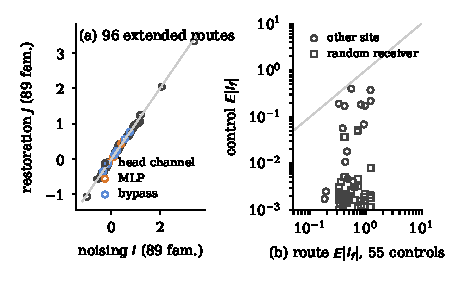
\includegraphics[width=\columnwidth]{figH_routes}
\caption{Route mapping on the 89 discovery families. (a) Noising against restoration
effect of the 96 extended configurations, by receiver type. (b) Mean absolute family
effect of each control against that of its target route (log axes); every control lies
below the diagonal.}
\label{fig:routes-app}
\end{figure}

\begin{table}[h]
\centering\scriptsize
\setlength{\tabcolsep}{3pt}
\begin{tabular}{@{}llrrr@{}}
\toprule
Source / site & Receiver / channel & $I_{89}$ & $J_{89}$ & $I_{69}$ \\
\midrule
L17H1 / union & L18H18 / V & $+3.400$ & $+3.335$ & $+3.391$ \\
L17H1 / union & L18H19 / V & $+2.074$ & $+2.054$ & $+2.057$ \\
L17H1 / union & L18H24 / V & $-1.004$ & $-1.070$ & $-0.988$ \\
L17H1 / union & L22H5 / V & $+0.898$ & $+0.865$ & $+0.882$ \\
L17H1 / union & L20H1 / V & $-0.582$ & $-0.576$ & $-0.567$ \\
L17H1 / union & L19H16 / V & $-0.247$ & $-0.225$ & $-0.243$ \\
L15H25 / child-last & L16H1 / V & $+0.182$ & $+0.187$ & $+0.182$ \\
L15H25 / child-last & L16H21 / V & $+0.210$ & $+0.223$ & $+0.215$ \\
L16H1 / colon & L18H18 / Q & $+0.372$ & $+0.370$ & $+0.367$ \\
L16H21 / colon & L18H18 / Q & $+0.349$ & $+0.407$ & $+0.348$ \\
L18H18 / colon & L27H6 / Q & $+0.662$ & $+0.663$ & $+0.674$ \\
L18H19 / colon & L27H6 / Q & $+0.731$ & $+0.742$ & $+0.736$ \\
L13H10 / sentence & L16H1 / V & $-0.175$ & $-0.175$ & $-0.172$ \\
L13H10 / sentence & L17H3 / V & $+0.150$ & $+0.139$ & $+0.151$ \\
L14H26 / sentence & L16H1 / V & $+0.136$ & $+0.140$ & $+0.139$ \\
L17H3 / colon & L18H18 / Q & $-0.158$ & $-0.172$ & $-0.155$ \\
L18H19 / colon & MLP 19 & $+0.532$ & $+0.554$ & $+0.514$ \\
L18H19 / colon & bypass & $+0.754$ & $+0.770$ & $+0.748$ \\
L18H18 / colon & bypass & $+0.547$ & $+0.562$ & $+0.546$ \\
L24H19 / colon & bypass & $+0.165$ & $+0.165$ & $+0.160$ \\
\bottomrule
\end{tabular}
\caption{Main retained routes: noising ($I$) and restoration ($J$) effects on the 89
discovery families and noising on the additional 69 families outside the common
subset. ``Union'' is the union of L17H1's mother-token, ``is'' and period masks;
``bypass'' tests the source's write reaching the answer without passing through a
tested head.}
\label{tab:routes-app}
\end{table}

\paragraph{S4.2 results: blocking, RI participation, backup.}
Table~\ref{tab:blocking-app} gives the receiver-blocking results and
Table~\ref{tab:ri31-app} the RI-participation audit for the 14 extended candidates.
The whole-group effects of the eight G1 groups overlap heavily because the
L18H18/L18H19 pair belongs to most of them (O1, O3, O4, I1, I2, I3); group differences
persist after same-order normalization, and the full-model gap itself depends on fact
order (14.6 vs.\ 7.8 logits). Donor and mean replacement can give very different
candidate accuracies (O3: 36.0\% vs.\ 97.8\% clean). In the backup test, L26H31 stays
below the retention rule in all five backgrounds (intact, $-$L21H18, $-\{$L21H18,
L22H5, L21H6$\}$, the same plus L27H6, and $-$L27H6: mean effect at most $+0.024$
logits, mean absolute at most $0.040$).

\begin{table}[h]
\centering\scriptsize
\setlength{\tabcolsep}{3pt}
\begin{tabular}{@{}llrrrr@{}}
\toprule
Source & Mask & $n_f$ & $J_W$ & $B$ & $B/J_W$ \\
\midrule
L17H1 & writer-union & 89 & $+5.358$ & $+4.790$ & 89.4\% \\
L17H1 & sentence & 89 & $+5.972$ & $+5.351$ & 89.6\% \\
L15H25 & child-last & 20 & $+0.457$ & $+0.442$ & 96.7\% \\
L15H25 & sentence & 20 & $+0.451$ & $+0.442$ & 97.8\% \\
L13H10 & sentence & 20 & $-0.330$ & $-0.429$ & 129.9\% \\
L17H3 & colon & 20 & $-0.417$ & $-0.304$ & 72.9\% \\
\bottomrule
\end{tabular}
\caption{Receiver blocking. $J_W$: restoration obtained by restoring the source's
clean activation at its mask in the corrupted run; $B$: the part of it lost when the
source's receivers (O3 for L17H1, O2 for L15H25, O1 for L13H10, O4 for L17H3) are
clamped to their corrupted colon outputs. Ratios are not exclusive mediation shares.}
\label{tab:blocking-app}
\end{table}

\begin{table}[h]
\centering\scriptsize
\setlength{\tabcolsep}{3pt}
\begin{tabular}{@{}lrrrrr@{}}
\toprule
Head & $I_{K}$ & $J_{K}$ & $I_{K,\mu}$ & $\mathbb{E}_f|I_{K,f}|$ & $I_K-I_0$ \\
\midrule
L18H19 & $+3.006$ & $+3.129$ & $+1.689$ & 3.006 & $-0.066$ \\
L22H5  & $+1.088$ & $+1.115$ & $+0.304$ & 1.088 & $+0.105$ \\
L16H21 & $+0.893$ & $+0.999$ & $+0.999$ & 0.899 & $-0.032$ \\
L16H1  & $+0.798$ & $+0.769$ & $+1.688$ & 0.803 & $-0.070$ \\
L17H24 & $+0.413$ & $+0.413$ & $+0.324$ & 0.413 & $-0.020$ \\
L19H16 & $-0.874$ & $-0.893$ & $-0.448$ & 0.874 & $-0.054$ \\
L23H15 & $-0.933$ & $-0.902$ & $-0.394$ & 0.933 & $+0.014$ \\
L26H23 & $-0.367$ & $-0.354$ & $-0.167$ & 0.376 & $+0.001$ \\
\midrule
L8H15  & $+0.284$ & $+0.316$ & $+0.130$ & 0.379 & $+0.005$ \\
L14H23 & $-0.215$ & $-0.201$ & $-0.134$ & 0.246 & $-0.003$ \\
L16H31 & $-0.173$ & $-0.167$ & $-0.261$ & 0.174 & $+0.014$ \\
L15H3  & $-0.104$ & $-0.086$ & $-0.154$ & 0.115 & $+0.002$ \\
L6H24  & $+0.096$ & $+0.103$ & $-0.065$ & 0.241 & $-0.005$ \\
L20H7  & $+0.032$ & $+0.099$ & $-0.177$ & 0.318 & $+0.058$ \\
\bottomrule
\end{tabular}
\caption{RI participation on the weakened background $K=\{$L21H18$\}$, 89 families:
noising ($I_K$) and restoration ($J_K$) with the corrupted donor, noising with mean
replacement ($I_{K,\mu}$), mean absolute family effect, and the change from the
intact-model single ($I_K-I_0$). Top: the eight strong RI heads; bottom: the six
conditional candidates retained for extension. Conditional participation is not a
newly unmasked backup for any head.}
\label{tab:ri31-app}
\end{table}

\paragraph{S4.3 local expansion (plan).}
Sources: L13H18 (three retained slot masks; receivers L16H1, L16H21, L18H18,
L18H19; K and V; MLP13, MLP14 or both released), L8H15 (two sentence masks; same
receivers; MLP8/MLP9), L16H31, L20H7 and L26H23 (colon sources; Q receivers in
later layers and residual continuation; local MLPs or blocks released), and two
chains (L15H25 $\to$ \{L16H1, L16H21\} $\to$ Q of L18H18/L18H19; L17H1 $\to$
\{L18H18, L18H19\} $\to$ Q of the late readers). 249 configurations before
deduplication; noising on 40 common pairs first, at most 9,960 endpoints plus at
most 2,240 matched direct comparators before reuse of compatible S4.1 records; at
most 16 retained contrasts extended to 178 pairs. TODO: executed panel.

\paragraph{S4.5 retention, reduction, completeness (plan).}
$C_0$ (33 heads) in eight disjoint reduction units---practical units, not
established functional modules: $W=\{$L15H25, L17H1$\}$; $D=\{$L16H1, L16H21$\}$;
$P=\{$L18H18, L18H19$\}$; $A=\{$L21H6, L21H18, L22H5, L27H6$\}$; $N=\{$L13H10,
L17H3, L18H24, L19H16, L20H1, L23H15, L26H23, L30H18$\}$; $R_6$ as above;
$T=\{$L14H26, L17H17, L17H24, L19H22, L21H23, L25H17, L30H13$\}$; $U=\{$L13H18,
L24H19$\}$. Acceptance: with $g_f(C)$ the family's clean-minus-corrupted gap,
\begin{align*}
F(C)&=\frac{\mathbb{E}_f\,g_f(C)}{\mathbb{E}_f\,g_f(\mathrm{full})}\in[0.8,1.2],\\
L(C)&=\frac{\mathbb{E}_f|g_f(C)-g_f(\mathrm{full})|}{\mathbb{E}_f|g_f(\mathrm{full})|}\le0.2,
\end{align*}
at most five points of candidate-accuracy loss in each condition and each order,
and the all-heads-mean baseline must not itself pass. Pre-declared addback if $C_0$
fails: the remaining 17 RI31 heads ($C_{50}$). Reduction: remove the unit whose
removal gives the smallest increase in $L$ while all guards hold, recompute the
remaining candidates in the new background, and allow at most two passes over the
units; evaluate the reduced mask on all 178 pairs and restore units in reverse
order if it fails. Completeness: remove $W,D,P,A,N$, the current RI members
($C\cap$RI31), the current non-RI members and $R_6$ from the full model and from
$C$ with identical masks. TODO: executed $C^*$ and guard values.

\paragraph{S4.4 fact $\times$ query panel (plan).}
Cells $x_{00}$ (clean), $x_{10}$ (fact swap), $x_{01}$ (query change), $x_{11}$
(both), with correct answers rebuilt from the fact table and a fixed $a{-}b$ scoring
sign in all four cells. Configurations: full model; full minus O3 (colon); full
minus the residual RI23 (all eligible test positions); retained $C^*$; $C^*$ minus
$C^*\cap$RI31; $C^*$ minus $C^*\setminus$RI31. Reported per configuration: the two
fact-axis and two query-axis contrasts, each cell's accuracy, and $B_D$. Panel: 20
common families, both orders; extension to the 89 families only if a core
condition-wise accuracy discrepancy between $C^*$ and the full model exceeds five
points or the sign of $B$ changes relative to the full model. Query-only changes
leave fact-site activations identical by causality, so the panel is a group-level
test. TODO: executed cells.

\section{Developmental check: details}
\label{app:dev}

\paragraph{Correspondence with \citet{ren2024semantic}.}
Same: the four task families (fruit/month and furniture/profession binary tasks, a
four-class fruit/month task, a nine-class fruit/animal/month task); the shot ladder
$\{0,1,2,3,4,5,10,20\}$ with class coverage enforced in the demonstrations when the
number of shots permits; the format-versus-pattern distinction; the AGENDA relation
set with seven relation types and entities reduced to single letters; the
developmental QK gate (argmax only) with $\tau{=}2.2$ as sensitivity; the
raw-embedding OV score. Adapted: accuracy is constrained to the legal task labels,
with vocabulary-wide format validity and legal-label probability mass reported
separately; inputs are relation-bearing sentences extracted from the corpus rather
than whole abstracts; rows are filtered for unambiguous single occurrences and
tokenizer-safe single-letter anchors under the OLMo-2 tokenizer, 60 self-relation
rows (source and target collapsing to the same entity) are excluded and listed, and
the assessment is balanced to 100 triplets per relation (700); the QK gate uses the
model's actual attention probabilities; the OV score is computed exactly on the
visible-token subset (the full-vocabulary softmax normalization cancels after
centring and in the ratio; verified numerically); the original spaCy function-word
removal is not applied (documented deviation); only the forward relation direction
is run. Per relation type, the 15 heads with the highest index are reported, with a
support requirement of at least ten scored events.

\paragraph{Checkpoints.}
Behaviour: 17 Stage-1 checkpoints of OLMo-2-1124-7B (steps 150, 600, 700, 850, 900,
1{,}000, 2{,}000, 3{,}000, 4{,}000, 6{,}000, 9{,}000, 19{,}000, 38{,}000, 76{,}000,
152{,}000, 357{,}000, 928{,}646; 1B to 3.9T tokens). Relation index: ten of these
(steps 150, 600, 700, 850, 900, 1{,}000, 2{,}000, 3{,}000, 9{,}000, 928{,}646).
The broad behavioural window (steps 600--1{,}000) was established before the index
timing was analysed; steps 700, 850 and 900 were added to the behavioural
measurement after the index sweep showed a routing maximum near step 850. The
850/900 localization is therefore targeted follow-up evidence rather than an
independent temporal prediction. Checkpoint identity is the exact optimizer step,
since OLMo's rounded token labels coincide for steps 600/700 and 850/900.

\paragraph{Behavioural metrics.}
Per task, shot count and checkpoint: constrained accuracy; gold-versus-best-wrong
margin; format validity (vocabulary-wide top token is a legal label); legal-label
probability mass; the 20-shot minus 1-shot accuracy gain; Wilson 95\% intervals
against task-specific chance; exact paired McNemar/binomial tests between adjacent
checkpoints on the reused prompt ids. The paired tests span 64 comparisons; raw
significance of some comparisons does not survive correction over that family, and
the report treats them as descriptive.

\begin{figure}[h]
\centering
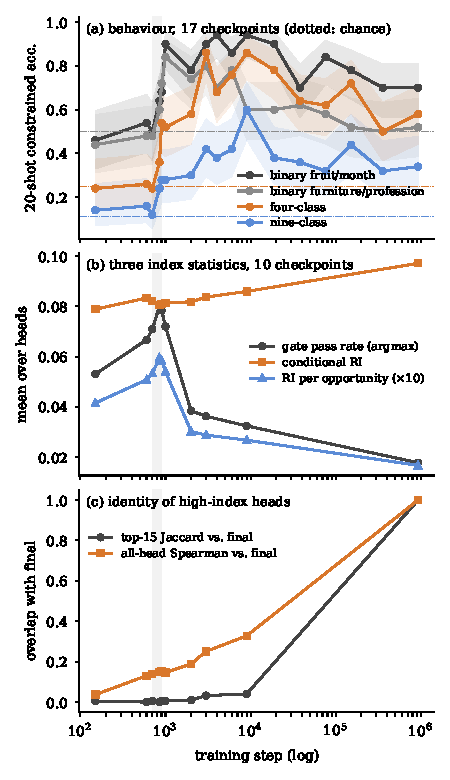
\includegraphics[width=\columnwidth]{figI_developmental}
\caption{Developmental measurements (shaded: steps 700--900). (a) 20-shot constrained
accuracy per task with Wilson intervals; dotted lines mark chance. (b) The three index
statistics averaged over all heads and relations at the ten RI checkpoints: the
argmax gate pass rate peaks near step 850 and then falls, the index per opportunity
follows it, and the conditional index rises slowly and monotonically. (c) Overlap of
each checkpoint's top-15 heads with the final checkpoint's (Jaccard) and all-head rank
correlation with the final checkpoint.}
\label{fig:dev-app}
\end{figure}

\paragraph{Index statistics.}
Per head and checkpoint: the index over gated events (conditional on the gate);
the gate pass rate under the argmax gate and under $\tau{=}2.2$; the index per
measurement opportunity (failed gates contribute zero), which combines frequency
and strength; and two null-target controls. Developmental changes in the
conditional index are tested on a fixed-support population (relation--head cells
with at least ten scored events at both endpoints) with a paired Bayesian cluster
bootstrap whose resampling unit is a cluster of text groups, not heads or events
(Dirichlet weights, 5,000 replicates); changes in pass rate use a paired cluster
bootstrap over the same units. Head stability: the top-$k$ heads at the final
checkpoint are traced backwards; per-checkpoint top-$k$ Jaccard overlap with the
final set and all-head rank correlation with the final checkpoint are reported.
Absence of a clear change in the conditional index is not evidence of no change,
and stability or instability of head identity is not a causal test of the heads'
role.


\end{document}
